\chapter{ANALISIS}
Pada bab ini akan dijelaskan analisis masalah penelitian ini. Analisis ini meliputi analisis masalah, eksplorasi spark, studi kasus, dan gambaran umum perangkat lunak.

\section{Analisis Masalah}
Berkembangnya penggunaan teknologi informasi menyebabkan data bertumbuh dengan sangat pesat. Istilah data yang memiliki ukuran yang besar dikenal sebagai \textit{big data}. \textit{Data mining} adalah cara untuk mengekstraksi sebuah informasi dari sekumpulan data untuk mendukung pengambilan keputusan atau pernyataan tertentu. Hasil \textit{data mining} yang mengandung data individu apabila disebarkan kepada pihak lain untuk kebutuhan tertentu tanpa dilakukan perlindungan privasi terlebih dahulu maka dapat melanggar hak privasi seseorang. Apabila informasi pribadi seseorang dapat diketahui oleh orang lain, maka mengakibatkan munculnya tindak kejahatan yang mengatasnamakan privasi orang bersangkutan. Oleh karena itu, perlu adanya sebuah cara untuk melindungi privasi seseorang sebelum dilakukan distribusi data.

\par Solusi yang tepat untuk menjamin perlindungan data sebelum dilakukan distribusi data adalah anonimisasi. Anonimisasi bertujuan untuk menyamarkan sebagian nilai atribut data yang unik terhadap atribut data lain, khususnya untuk atribut yang termasuk dalam kategori atribut privasi menurut PII. \textit{Privacy-preserving data mining} adalah sebuah cara untuk melindungi data sebelum dilakukan data mining agar privasi dari hasil data mining dapat terlindungi. \textit{K-anonymity} adalah salah satu metode agar \textit{privacy-preserving data mining} dapat dicapai dengan menyamarkan beberapa nilai atribut data. Tujuan utama dari penelitian ini adalah mempelajari, menganalisis, melakukan eksperimen, membuat perangkat lunak terkait anonimisasi pada lingkungan big data, dan menguji hasilnya agar privasi data dapat terjaga. Berikut beberapa kajian yang akan dianalisis terkait teknik anonimisasi pada lingkungan \textit{big data}.

\subsection{Dataset Eksperimen}
Dataset yang dipakai adalah \textit{Adult}. Dataset ini diperoleh dari website Kaggle. Dataset ini disimpan dalam format CSV seperti penjelasan pada bagian \ref{theory:csv}. Format CSV memisahkan nilai atribut data melalui simbol koma. Dataset \textit{Adult} dipilih, karena pernah digunakan sebelumnya untuk eksperimen algoritma \textit{k-anonymity}. Dataset ini berisi sampel sensus penduduk di Amerika Serikat pada tahun 1990. Penelitian ini melibatkan 10 juta baris data dengan ukuran data sebesar 1.2 GB. 

\begin{lstlisting}[basicstyle=\ttfamily, frame=single,
	columns=fullflexible, keepspaces=true, breaklines=true, label=lst:lst_csv, caption=Dataset Adult]
age,workclass,zip,education,year_of_education,marital_status,occupation
39,State-gov,77516,Bachelors,13,Never-married,Adm-clerical
50,Self-emp-not-inc,83311,Bachelors,13,Married-civ-spouse,Exec-managerial
38,Private,215646,HS-grad,9,Divorced,Handlers-cleaners
53,Private,234721,11th,7,Married-civ-spouse,Handlers-cleaners
28,Private,338409,Bachelors,13,Married-civ-spouse,Prof-specialty
\end{lstlisting}

\noindent Berikut adalah kemungkinan nilai untuk masing-masing jenis atribut dalam dataset:

\begin{itemize}
\item Age: numerik

\item Workclass: \textit{Private, Self-emp-not-inc, Self-emp-inc, Federal-gov, Local-gov, State-gov, Without-pay, Never-worked.}

\item Education: \textit{Bachelors, Some-college, 11th, HS-grad, Prof-school, Assoc-acdm, Assoc-voc, 9th, 7th-8th, 12th, Masters, 1st-4th, 10th, Doctorate, 5th-6th, Preschool.}

\item Years of education: numerik

\item Marital status: 
\textit{Married-civ-spouse, Divorced, Never-married, Separated, Widowed, Married-spouse-absent, MarriedAF-spouse}

\item Occupation: \textit{Tech-support, Craft-repair, Other-service, Sales, Exec-managerial, Prof-specialty, Handlers-cleaners, Machine-op-inspect, Adm-clerical, Farming-fishing, Transport-moving, Priv-house-serv, Protective-serv, ArmedForces.}

\item Relationship: \textit{Wife, Own-child, Husband, Not-in-family, Other-relative, Unmarried}

\item Race: \textit{White, Asian-Pac-Islander, Amer-Indian-Eskimo, Other, Black}

\item Sex: \textit{Male, Female}

\item Capital gain: numerik

\item Capital loss: numerik

\item Hours per week: numerik

\item Native country: \textit{United-States, Cambodia, England, Puerto-Rico, Canada, Germany, Outlying-US, India, Japan, Greece, South, China, Cuba, Iran, Honduras, Philippines, Italy, Poland, Jamaica, Vietnam, Mexico, Portugal, Ireland, France, Dominican-Republic, Laos, Ecuador, Taiwan, Haiti, Columbia, Hungary, Guatemala, Nicaragua, Scotland, Thailand, Yugoslavia, El-Salvador, Trinidad and Tobago, Peru, Hong, HollandNetherlands}

\item Income: $\leq$50K, $>$50K
\end{itemize}


\subsection{\textit{Personally Identifiable Information}}
Pada bagian \ref{sec:privasi}, telah dijelaskan mengenai konsep \textit{Personally Identifiable Information} (PII). PII digunakan untuk mengelompokkan nilai atribut berdasarkan kategori atribut yang digunakan pada proses anonimisasi data. Berdasarkan bagian \ref{sec:anonimisasi}, atribut pada proses anonimisasi dapat dikategorikan sebagai \textit{identifier, quasi-identifier}, dan \textit{sensitive attribute}. 
\par Atribut \textit{identifier} adalah atribut yang dapat mengidentifikasi individu secara langsung. Contoh dari atribut identifier pada dataset \textit{Adult} adalah nama, tempat tanggal lahir, alamat rumah, nomor KTP. Atribut \textit{quasi-identifier} adalah atribut yang dapat mengidentifikasi seseorang apabila nilai sebuah atribut digabung dengan nilai atribut lain pada baris data yang sama. Contoh \textit{quasi-identifier} pada dataset \textit{Adult} adalah \textit{age, zip, education, years of education, occupation, race, sex, native country}. \textit{Sensitive attribute} adalah nilai yang ingin dirahasiakan. Contoh sensitive attribute pada dataset \textit{Adult} adalah \textit{workclass, marital status, relationship, income}.
\par Atribut \textit{identifier} nantinya akan dihilangkan sebelum dilakukan proses anonimisasi, karena nilai dari atribut \textit{identifier} dapat langsung mengidentifikasi seseorang. Sedangkan \textit{sensitive attribute} nilainya tidak akan dihapus karena akan melalui proses anonimisasi bersamaan dengan nilai dari \textit{quasi-identifier} sehingga \textit{sensitive attribute} milik individu tidak dapat dibedakan satu sama lain pada hasil tabel akhir anonimisasi sehingga keamanan  distribusi data terjamin.


\subsection{Perhitungan \textit{Distance} dan \textit{Information Loss}}
Pada bagian \ref{theory:dist,il,cf}, telah dijelaskan konsep mengenai penggunaan \textit{distance} dan \textit{information loss}. \textit{Distance} dan \textit{Information Loss} digunakan oleh algoritma \textit{Greedy k-member clustering} untuk mencari kelompok data terbaik sehingga menghasilkan pengelompokkan data yang tepat. 

\subsubsection{\textit{Distance}}
\textit{Distance} bertujuan untuk menentukan hasil pengelompokan data pada algoritma \textit{Greedy k-member clustering}. Pemilihan distance yang baik dapat mencapai hasil klasifikasi yang lebih optimal.
\\\\
\noindent Akan diambil 2 sampel data dari dataset \textit{Adult} sebagai berikut:
\begin{enumerate}
\item 39, State-gov, 77516, Bachelors, 13, Never-married, Adm-clerical, Not-in-family, White, Male, 2174, 0, 40, United-States, <=50K
\item 50, Self-emp-not-inc, 83311, Bachelors, 13, Married-civ-spouse, Exec-managerial, Husband, White, Male, 0, 0, 13, United-States, <=50K
\end{enumerate}

\noindent \textit{Distance} atribut numerik dapat dihitung sebagai berikut berdasarkan umur data pertama ($v_1$)= 39, umur data kedua ($v_2$)= 50, dan jumlah data ($D$)= 10.000.000 data.
\begin{align*}
\delta_n(v_1,v_2) &= \frac{|v_1 - v_2|}{|D|}
= \frac{|39 - 50|}{10.000.000}\vspace{0.2cm}
= \frac{11}{10.000.000}\vspace{0.2cm}
= 0.0000011
\end{align*}

\noindent \textit{Distance} atribut kategorikal dapat dihitung sebagai berikut berdasarkan \textit{workclass} data pertama ($v_1$)= \textit{State-gov, workclass} data kedua ($v_2$)= \textit{Self-emp-not-inc}, jumlah subtree ($H(\Lambda(v_i,v_j))$)= 1, dan tinggi taxonomy tree ($H(T_D)$)= 1  seperti pada Gambar \ref{fig:TD}.
\begin{align*}
\delta_C(v_1,v_2) = \frac{H(\Lambda(v_i,v_j))}{H(T_D)} 
= \frac{1}{1}
= 1
\end{align*}

\begin{figure}[H]
	\centering
	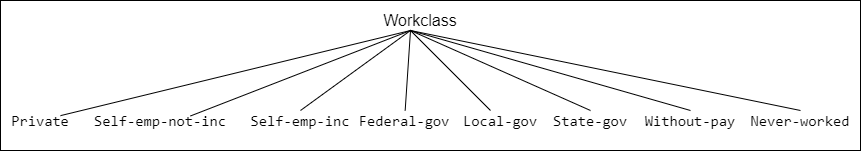
\includegraphics[scale=0.4]{TD}
	\caption{Taxonomy Tree (Workclass)}
	\label{fig:TD}
\end{figure}

\subsubsection{\textit{Information Loss}}
\textit{Information Loss} (IL) bertujuan untuk mengevaluasi seberapa baik kinerja algoritma \textit{k-anonymity} terhadap nilai informasi sebuah data. Tabel  \ref{table:informationloss} adalah contoh hasil pengelompokan data pada dataset \textit{Adult}:

\begin{table}[H]
\centering
\caption{Tabel Hasil Clustering Data pada Cluster 1}
\begin{tabular}{c c c c c c c c}
\hline 
Age & Workclass & Education & Occupation & Sex & Income & Cluster Name \\ 
\hline 
39 & State-gov & Bachelors & Adm-clerical & Male & <=50K & Cluster 1 \\ 
50 & Self-emp-not-inc & Bachelors & Exec-managerial & Male & <=50K & Cluster 1 \\ 
38 & Private & HS-grad & Handlers-cleaners & Male & <=50K & Cluster 1 \\ 
53 & Private & 11th & Handlers-cleaners & Male & <=50K & Cluster 1 \\ 
28 & Private & Bachelors & Prof-specialty & Female & <=50K & Cluster 1 \\ 
\hline 
\end{tabular} 
\label{table:informationloss}
\end{table}

\noindent \textit{Information Loss} (IL) dapat dihitung sebagai berikut berdasarkan atribut numerik yaitu jumlah anggota \textit{cluster} ($e$)= 5, $MAX_{Age}$= 53, $MIN_{Age}$= 28, $N_Age$= 5 mencakup atribut \textit{Age} dan atribut kategorikal yaitu $H(\Lambda(\cup_{C_j}))$= 1, $H(T_{C_j})$= 1.
\begin{align*}
D(e) &= \sum_{i=1}^{m} \frac{(MAX_{N_i} - MIN_{N_i})}{|N_i|} + \sum_{j=1}^{n}\frac{H(\Lambda(\cup_{C_j}))}{H(T_{C_j})}\\
&= \frac{(53 - 28)}{5} + \frac{1}{1}+\frac{1}{1}+\frac{1}{1}+\frac{1}{1}+\frac{1}{1} = 10\\\\
IL(e) &= |e| \cdot D(e)\\
&= 5 \cdot 10 = 50
\end{align*}

\noindent Total \textit{Information Loss} dihitung dari jumlah \textit{Information Loss} masing-masing \textit{cluster}.
\begin{align*}
Total-IL(AT) &= \sum_{e \in \varepsilon}^{}  IL(e)\\
&= IL(cluster1)+IL(cluster2)+\ldots+IL(clusterN)
\end{align*}

\subsection{\textit{Greedy K-Member Clustering}}
Algoritma \textit{Greedy k-member clustering} telah dijelaskan pada bagian \ref{sec:greedyclustering}. Algoritma ini bertujuan untuk membagi seluruh data pada tabel terhadap masing-masing \textit{cluster} untuk kompleksitas yang lebih baik dan mendukung nilai utilitas informasi yang lebih baik dibandingkan algoritma \textit{clustering} lain. Pada bagian ini, akan dilakukan eksperimen sederhana untuk mencari tahu langkah kerja algoritma \textit{Greedy k-member clustering} secara konseptual.

\par Melalui sampel data pada Tabel \ref{table:adults}, akan diputuskan nilai dari setiap atribut anonimisasi. Jenis atribut anonimisasi yang pertama adalah Quasi-identifier, dengan nilai QI = \{\textit{Age, Education, Occupation, Sex, Income}\}. Jenis atribut anonimisasi yang kedua adalah Sensitive Attribute, dengan nilai SA = \{\textit{Workclass}\}. Jika telah diketahui tabel data seperti diatas, k = 2, dan jumlah cluster (m) = 2, maka algoritma ini siap ditelusuri lebih lanjut.

\begin{table}[H]
\centering
\caption{Dataset Adults}
\begin{tabular}{c c c c c c c c}
\hline 
ID & Age & Workclass & Education & Occupation & Sex & Income\\ 
\hline 
t1 & 39 & State-gov & Bachelors & Adm-clerical & Male & <=50K \\ 

t2 & 50 & Self-emp-not-inc & Bachelors & Exec-managerial & Male & <=50K  \\ 

t3 & 38 & Private & HS-grad & Handlers-cleaners & Male & <=50K  \\ 

t4 & 53 & Private & 11th & Handlers-cleaners & Male & <=50K  \\ 
 
t5 & 28 & Private & Bachelors & Prof-specialty & Female & <=50K	 \\ 
\hline 
\end{tabular} 
\label{table:adults}
\end{table}

\noindent Berikut adalah tahapan yang terjadi pada algoritma \textit{Greedy k-member clustering}:

\begin{enumerate}
\item Nilai awal result = $\emptyset$, $r = \{t1\}$, $|S|$ = 5, $k = 2$
\item Karena kondisi $|S| \geq k$ terpenuhi, maka dilakukan perulangan sebagai berikut:
\begin{enumerate}
\item Nilai r diubah menjadi r = \{t3\}, karena terbukti data t3 memiliki $\Delta(t1,t3)=1.7189$ yang paling tinggi dari seluruh \textit{distance} lain. Berikut adalah contoh perhitungannya:
\begin{align*}
\Delta (t_1,t_2) = 1.715\\
\Delta (t_1,t_3) = 2.431\\
\Delta (t_1,t_4) = 2.122\\
\Delta (t_1,t_5) = 1.621 
\end{align*}
\item Nilai awal S = \{t1, t2, t4, t5\}
\item Nilai awal c = \{t3\}, |c| = 1
\item Karena kondisi |c| < k terpenuhi, maka dilakukan perulangan sebagai berikut:

\begin{enumerate}
\item Nilai r diubah menjadi r = \{t3,t4\}, karena terbukti data t4 memiliki $IL(t3 \cup t4)=0.330$ yang paling rendah dari seluruh data lain. Berikut adalah contoh perhitungannya:
\begin{align*}
IL(t3 \cup t1) = 0.479 \\
IL(t3 \cup t2) = 0.515 \\
IL(t3 \cup t4) = 0.330 \\
IL(t3 \cup t5) = 0.367 
\end{align*}
\item Nilai S diubah menjadi S = \{t1, t2, t5\}, |S| = 4
\item Nilai c ditambahkan menjadi c = \{t3, t4\}, |c| = 2

\end{enumerate}
\item Karena kondisi |c| < k sudah tidak terpenuhi lagi, maka perulangan ini akan berhenti
\item Nilai \textit{result} akan ditambahkan menjadi result = \{t3, t4\}
\item Karena kondisi $|S| \geq k$ masih terpenuhi, maka perulangan akan tetap berlanjut sampai pada kondisi dimana $|S| < k$ sehingga hasil akhirnya adalah \textit{result} = \{\{t3, t4\}, \{t2, t5\}\}, S = \{t1\}, |S| = 1

\end{enumerate}

\item Karena kondisi $S \neq 0$ terpenuhi, maka dilakukan perulangan sebagai berikut:

\begin{enumerate}
\item Nilai r diubah menjadi r = \{t1\}
\item Nilai S diubah menjadi S = $\{\phi\}$, |S| = 0
\item Nilai c diubah menjadi c = \{t3, t4\} karena terbukti \textit{cluster} c memiliki $IL(\{t3,t4\} \cup t1)=0.279$ yang paling rendah dari seluruh \textit{cluster} lain. Berikut adalah contoh perhitungannya:
\begin{align*}
IL(\{t3,t4\} \cup t1) = 0.279 \\
IL(\{t2,t5\}\cup t1) = 0.515 \\
\end{align*}
\item Nilai c ditambahkan menjadi c = \{t1, t3, t4\}
\item Nilai c pada perulangan ini tidak akan ditambahkan pada \textit{result}, karena telah ditetapkan k = 2 sedangkan jumlah datanya ganjil, sehingga sisa data tersebut tidak akan dicatat pada variabel \textit{result} agar menjaga masing-masing \textit{cluster} hanya memiliki 2 anggota saja.
\item Karena kondisi $S \neq 0$ sudah tidak terpenuhi lagi, maka perulangan ini akan berhenti.

\end{enumerate}

\item Hasil akhirnya adalah result = \{\{t3, t4\}, \{t2, t5\}\} dikembalikan sebagai output untuk algoritma \textit{Greedy k-member clustering} seperti pada Tabel \ref{table:greedykmember} sebagai berikut:
\begin{table}[H]
\centering
\caption{Tabel Hasil Greedy K-Member Clustering}
\begin{tabular}{c c c c c c c c}
\hline 
ID & Age & Workclass & Education & Occupation & Sex & Income\\ 
\hline 
t3 & 38 & Private & HS-grad & Handlers-cleaners & Male & <=50K  \\ 
t4 & 53 & Private & 11th & Handlers-cleaners & Male & <=50K  \\ 
\hline 
t2 & 50 & Self-emp-not-inc & Bachelors & Exec-managerial & Male & <=50K  \\ 
t5 & 28 & Private & Bachelors & Prof-specialty & Female & <=50K	 \\ 
\hline 
\end{tabular} 
\label{table:greedykmember}
\end{table}

\end{enumerate}

\subsection{\textit{Domain Generalization Hierarchy}}
Pada bagian \ref{theory:hierarchy_generalization}, telah dijelaskan konsep mengenai \textit{Hierarchy Based Generalization}. DGH adalah contoh penerapan dari \textit{Hierarchy Based Generalization}. DGH bertujuan untuk melindungi data dengan cara menerapkan metode generalisasi terhadap nilai atribut data yang bersifat unik, agar menjadi nilai yang lebih umum. Berikut adalah penerapan DGH terhadap dataset \textit{Adult}. \\

\noindent Diketahui kemungkinan nilai unik atribut pada dataset \textit{Adult} sebagai berikut:

\begin{itemize}
\item Age = \{33,36,38,40,42,43,46,49\}
\item ZIP = \{77516,77517,77526,77527\}
\item Sex = \{Male,Female\}
\end{itemize}

\noindent Nilai atribut ZIP, akan dibangun tiga jenis domain sebagai berikut:

\begin{itemize}
\item Domain dengan nilai kurang spesifik\\
Domain ini dipilih apabila tujuannya adalah lebih mengutamakan hasil informasi yang diperoleh dengan cara melakukan sedikit anonimisasi pada nilai data. Contohnya atribut ZIP akan diubah menjadi \{7751*,7752*\} apabila satu digit terakhir memiliki nilai yang berbeda dan digit sisanya memiliki nilai yang sama.
\item Domain dengan nilai yang lebih umum\\
Domain ini dipilih apabila tujuannya adalah menyeimbangkan nilai informasi yang diperoleh dengan tingkat perlindungan data yang didapat dengan cara meningkatkan level anonimisasi nilai data. Contohnya atribut ZIP akan diubah menjadi \{775**\} apabila kedua digit terakhir memiliki nilai yang berbeda dan digit sisanya memiliki nilai yang sama.
\item Domain dengan nilai yang umum.
Domain ini dipilih apabila tujuannya adalah mengutamakan perlindungan data. Biasanya jenis domain ini jarang dipilih, karena hasil anonimisasinya tidak dapat digunakan untuk proses data mining (memiliki nilai akurasi yang rendah apabila dilakukan pemodelan \textit{data mining}). Contohnya atribut ZIP akan diubah menjadi \{*****\}

\end{itemize}

\begin{figure}[H]
	\centering
	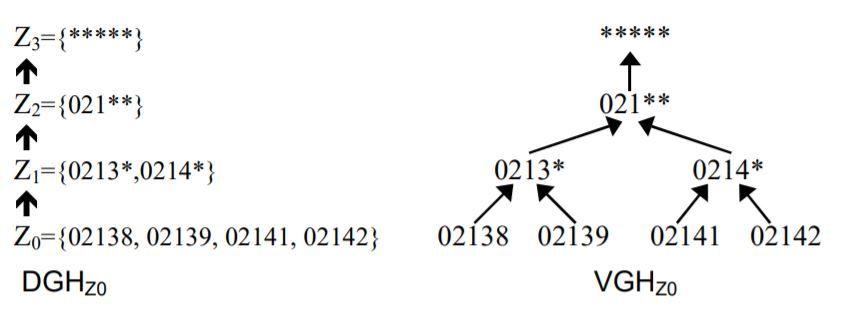
\includegraphics[scale=0.55]{DGH1}
	\caption{DGH dan VGH pada atribut ZIP}
	\label{fig:DGH1}
\end{figure}

\noindent Nilai atribut \textit{Age} akan dibangun berdasarkan ketentuan berikut: 

\begin{itemize}
\item Nilai atribut \textit{Age} akan diubah menjadi rentang nilai. Contohnya nilai 33  diubah menjadi [30-39], karena 33 termasuk pada rentang nilai tersebut.
\end{itemize}

\noindent Nilai atribut \textit{Age} dan \textit{Sex} akan dibangun berdasarkan ketentuan berikut: 

\begin{itemize}
\item Nilai atribut \textit{Sex} termasuk nilai kategorikal, sehingga akan diubah menjadi nilai yang lebih umum. Contohnya nilai \textit{Male/Female} diubah menjadi \textit{Person} (bentuk umum).
\end{itemize}


\newpage
\subsection{\textit{K-Anonymity}}
Pada bagian \ref{sec:anonimisasi}, dijelaskan konsep anonimisasi. \textit{K-anonymity} bertujuan untuk menyamarkan nilai dari masing \textit{quasi-identifier} yang unik pada kelompok \textit{cluster} yang sama. Kata kuncinya adalah nilai unik pada kelompok \textit{cluster} yang sama. Setelah dataset dilakukan anonimisasi, maka data privasi sudah terlindungi sehingga publikasi data dapat dilakukan dengan aman. Tabel \ref{table:clustering} adalah kelompok data yang dihasilkan oleh algoritma \textit{Greedy k-member clustering}. 
\begin{table}[H]
\centering
\caption{Tabel Hasil Clustering}
\begin{tabular}{c c c c c c c c}
\hline 
ID & Age & Workclass & Education & ZIP & Sex & Hours/week & Cluster Name\\ 
\hline 
t3 & 32 & Private & HS-grad & 77516 & Male & 30 & Cluster 1 \\ 
t4 & 32 & Private & 11th & 77541 & Female & 30 & Cluster 1 \\ 
\hline 
t2 & 34 & Self-emp-not-inc & Bachelors & 77526 & Male & 34 & Cluster 2 \\ 
t5 & 50 & Private & Bachelors & 77526 & Male & 37	& Cluster 2\\ 
\hline 
t1 & 47 & Local-gov & Bachelors & 77581 & Male & 54 & Cluster 3\\ 
t6 & 50 & Federal-gov & HS-grad & 77532 & Male & 57 & Cluster 3\\ 
\hline 
\end{tabular} 
\label{table:clustering}
\end{table}
\vspace{0.4cm}

\noindent Diketahui bentuk generalisasi berdasarkan \textit{Domain Generalization Hierarchy} sebagai berikut:
\begin{align*}
Age &= \{[20-30], [40-50]\}\\
ZIP &= \{775**\}\\
Sex &= \{Person\}\\
Hours/week &=\{[12-18], [33-37], [53-61]\}
\end{align*} 

\vspace{0.2cm}
\noindent Berikut adalah tahapan proses anonimisasi dengan model \textit{k-anonymity}:
\begin{enumerate}

\item Diketahui \textit{quasi-identifier} sebagai berikut QI = \{\textit{Age, ZIP, Sex, Hours/week}\} dan \textit{sensitive attribute} sebagai berikut SA = \{\textit{Workclass, Education}\}

\item Mencari nilai \textit{quasi-identifier} yang unik pada kelompok \textit{cluster} yang sama. Sebagai contoh, \textit{cluster 2} memiliki nilai \textit{quasi-identifier} yang unik sebagai berikut QI = \{\textit{Age, Hours/week}\}

\item Melakukan generalisasi DGH pada nilai \textit{quasi-identifier} yang unik menjadi bentuk. Sebagai contoh, QI = \{\textit{Age, Hours/week}\} memiliki nilai yang unik, sehingga diubah menjadi \textit{Age} = \{[40-50]\}, \textit{Hours/week} = \{[33-37]\}

\item \textit{Sensitive attribute} tidak akan dilakukan generalisasi, karena \textit{quasi-identifier} sudah dilakukan generalisasi sehingga seseorang akan sulit untuk menebak kepemilikan dari \textit{sensitive attribute}.

\item Ulangi hal yang sama pada langkah sebelumnya untuk setiap \textit{cluster}. Hasil akhir dari proses anonimisasi ada pada Tabel \ref{table:anonimisasi} sebagai berikut: 
\begin{table}[H]
\centering
\caption{Tabel Hasil Anonimisasi}
\begin{tabular}{c c c c c c c c}
\hline 
ID & Age & Workclass & Education & ZIP & Sex & Hours/week & Cluster Name\\ 
\hline 
t3 & 32 & Private & HS-grad & 775** & Person & 30 & Cluster 1 \\ 
t4 & 32 & Private & 11th & 775** & Person & 30 & Cluster 1 \\ 
\hline 
t2 & [40-50] & Self-emp-not-inc & Bachelors & 77526 & Male & [33-37] & Cluster 2 \\ 
t5 & [40-50] & Private & Bachelors & 77526 & Male & [33-37]	& Cluster 2\\ 
\hline 
t1 & [40-50] & Local-gov & Bachelors & 775** & Male & [53-61] & Cluster 3\\ 
t6 & [40-50] & Federal-gov & HS-grad & 775** & Male & [53-61] & Cluster 3\\ 
\hline 
\end{tabular} 
\label{table:anonimisasi}
\end{table}

\end{enumerate}

\newpage
\section{Eksplorasi Spark}
Pada bagian ini akan dilakukan penelusuran lebih lanjut mengenai beberapa hal penting terkait Spark sebelum melakukan eksperimen metode anonimisasi pada Spark.\\ 

\noindent Berikut adalah beberapa hal penting terkait Spark:
\begin{itemize}

\item Spark bekerja sama dengan komponen lain seperti JDK, SBT, HDFS sehingga instalasi Spark untuk masing-masing sistem operasi dapat berbeda. Pada penelitian in, akan dilakukan instalasi Spark melalui sistem operasi Windows. 

\item Spark dapat bekerja dengan bahasa pemrograman Scala. Scala dipilih karena memiliki efektivitas yang baik pada penulisan kode program. Scala dapat menyederhanakan perintah pada Spark menjadi baris yang lebih sedikit.

\item Program Spark dijalankan dengan cara membuat jar sebelum perintah eksekusi dijalankan. Hal ini menghambat perkerjaan pada tahap implementasi perangkat lunak. Intel IJ adalah sebuah \textit{Integrated Development Environment} (IDE) yang memfasilitasi pemrograman Scala pada Spark dan menampilkan hasil pemrosesan Spark  secara langsung.

\item Spark menyediakan konfigurasi untuk mengatur jumlah resource  yang dibutuhkan (jumlah pemakaian RAM, \textit{core} CPU) pada pemrosesan data. Konfigurasi ini bertujuan agar Spark dapat mengolah data yang besar secara maksimal dengan menggunakan jumlah \textit{resource} yang tersedia. Konfigurasi ini ditulis pada perintah eksekusi Spark.
 

\end{itemize}



\subsection{Instalasi Spark}
Spark berjalan pada sistem operasi Windows, Linux, dan Mac OS. Spark dapat dijalankan secara lokal menggunakan satu komputer, meskipun Spark tetap membutuhkan beberapa komputer untuk pemrosesan data yang besar. Jenis instalasi Spark dijelaskan pada bagian \ref{sec:instalasi_spark}. Pada penelitian ini digunakan jenis instalasi Standalone untuk Spark versi 2.4.5 pada sistem operasi Windows. Sebelum melakukan instalasi Spark, ada beberapa hal yang harus diperhatikan dan dipenuhi. 
\\\\
\noindent Berikut adalah beberapa hal yang harus diperhatikan:

\begin{itemize}
\item Java 7, Python 2.6 telah dihilangkan pada implementasi Spark 2.2.0 ke atas.
\item Scala 2.10 sudah usang apabila dipakai pada Spark 2.4.1 ke atas.
\item Hadoop 2.6.5 telah dihilangkan pada implementasi Spark 2.2.0 ke atas.
\end{itemize}

\noindent Berikut adalah beberapa hal yang harus dipenuhi:

\begin{itemize}
\item Spark 2.4.5 dapat berjalan di Java 8, Python 2.7+/3.4+ dan R 3.1+ 
\item Spark 2.4.5 dapat menggunakan Scala 2.12
\item Spark 2.4.5 dapat menggunakan Hadoop 2.7
\end{itemize}

\noindent Berikut adalah tahapan instalasi Spark 2.4.5 secara umum:

\begin{enumerate}
\item Melakukan instalasi Java 8.
\item Melakukan instalasi Spark 2.4.5
\item Melakukan instalasi IntelIJ untuk Scala sbt.
\end{enumerate}

\newpage
\subsubsection{Instalasi Java 8}
\noindent Berikut adalah tahapan instalasi Java 8 secara lengkap:

\begin{enumerate}

\item Download Java SE Development Kit 8u31 pada link berikut \path{https://www.oracle.com/technetwork/java/javase/downloads/java-archive-javase8-2177648.html}
 
\item Lakukan instalasi Java SE Development Kit 8u31 seperti biasa.

\item Pilih menu \textit{Edit the system environment variables}.

\item Buat \textit{environment variables} baru seperti Gambar \ref{fig:instal_java_5}.

\begin{figure}[H]
	\centering
	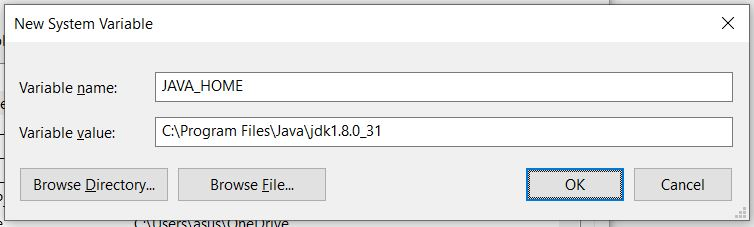
\includegraphics[scale=0.7]{instal_java_5}
	\caption{Environment Variables}
	\label{fig:instal_java_5}
\end{figure}


\item Tambahkan \path{%JAVA_HOME%\bin;} pada Path di System variables seperti Gambar \ref{fig:spark_instal_5}.

\begin{figure}[H]
	\centering
	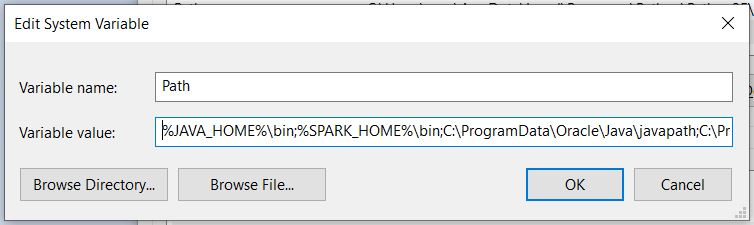
\includegraphics[scale=0.8]{spark_instal_5}
	\caption{Penambahan Variable Value}
	\label{fig:spark_instal_5}
\end{figure}


\end{enumerate}

\noindent Berikut adalah tahapan verifikasi terhadap instalasi Java 8:

\begin{enumerate}

\item Pilih menu \textit{command prompt}.

\item Jalankan perintah java -version pada Command Prompt.

\begin{figure}[H]
	\centering
	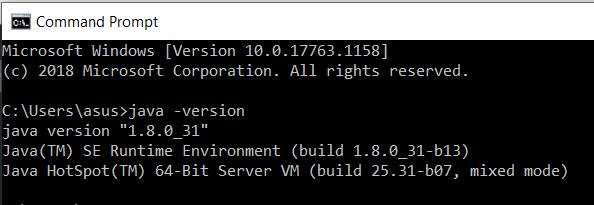
\includegraphics[scale=0.8]{instalasi_java}
	\caption{Perintah java -version}
	\label{fig:instalasi_java}
\end{figure}

\item Apabila sistem tidak menampilkan pesan error, maka Java 8 sudah terpasang dengan baik.

\end{enumerate}

\newpage
\subsubsection{Instalasi Spark 2.4.5}
Berikut adalah tahapan instalasi Spark 2.4.5 secara lengkap:
\begin{enumerate}

\item Download winutils.exe dari link \path{https://github.com/steveloughran/winutils/tree/master/hadoop-2.7.1/bin}, tempatkan winutils.exe pada \path{C:\winutils\bin}


\item Download Spark 2.4.5 dari link \path{https://downloads.apache.org/spark/spark-3.0.0-preview2/spark-3.0.0-preview2-bin-hadoop2.7.tgz}

\item Buat folder sebagai berikut \path{C:\spark-2.4.4} dan ekstraksi \textit{file} \path{spark-2.4.5-bin-hadoop2.7.tgz} di dalam folder tersebut.

\item Buat \textit{environment variables} baru seperti Gambar \ref{fig:spark_instal_3}.

\begin{figure}[H]
	\centering
	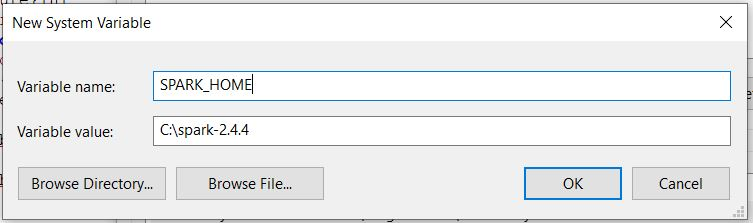
\includegraphics[scale=0.6]{spark_instal_3}
	\caption{Environment Variable}
	\label{fig:spark_instal_3}
\end{figure}

\item Tambahkan \path{%SPARK_HOME%\bin;} pada Path di System variables sepertin Gambar \ref{fig:spark_instal_5}

\begin{figure}[H]
	\centering
	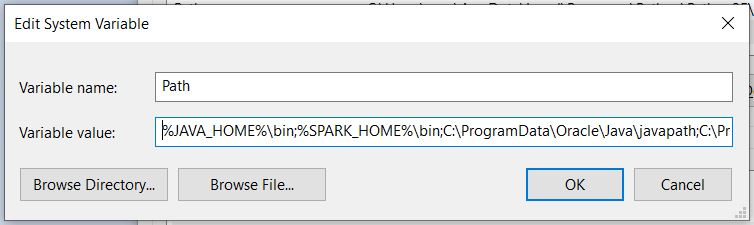
\includegraphics[scale=0.6]{spark_instal_5}
	\caption{Penambahan Variable Value}
	\label{fig:spark_instal_5}
\end{figure}

\end{enumerate}

\noindent Berikut adalah tahapan verifikasi terhadap instalasi Spark 2.4.5:
\begin{enumerate}
\item Jalankan perintah \path{spark-shell} pada \textit{command prompt}.

\item Apabila terminal menampilkan tampilan seperti pada Gambar \ref{fig:spark_instal_7}, artinya Spark 2.4.5 sudah dapat berjalan dengan baik pada komputer tersebut.

\begin{figure}[H]
	\centering
	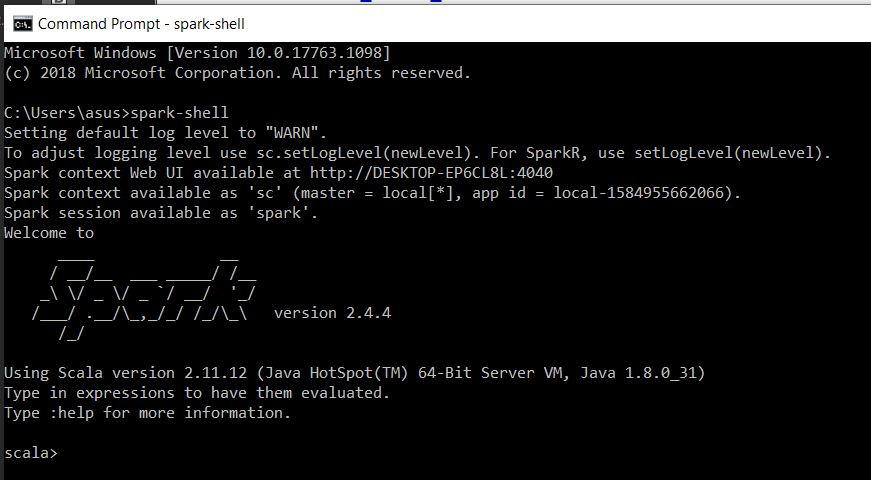
\includegraphics[scale=0.55]{spark_instal_7}
	\caption{Spark 2.4.5}
	\label{fig:spark_instal_7}
\end{figure}

\end{enumerate}

\newpage
\subsubsection{Instalasi IntelIJ untuk Scala SBT}
Berikut adalah tahapan instalasi IntelIJ:

\begin{enumerate}
\item Download IntelIJ melalui link berikut \\
\path{https://www.jetbrains.com/idea/download/#section=windows}

\item Lakukan instalasi IntelIJ seperti biasa.
\begin{figure}[H]
	\centering
	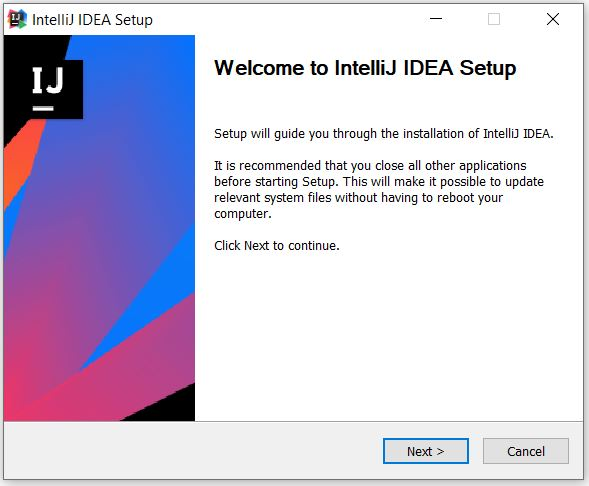
\includegraphics[scale=0.65]{intelij_install}
	\caption{Instalasi IntelIJ}
	\label{fig:intelij_install}
\end{figure}

\end{enumerate}

\noindent Berikut adalah tahapan pemasangan \textit{plugin} Scala pada IntelIJ.

\begin{enumerate}

\item Pilih menu \textit{Configure} pada IntelIJ, lalu pilih menu \textit{Plugins}.

\item Telusuri \textit{plugin} Scala pada kolom pencarian seperti Gambar \ref{fig:intelij_2}.
\begin{figure}[H]
	\centering
	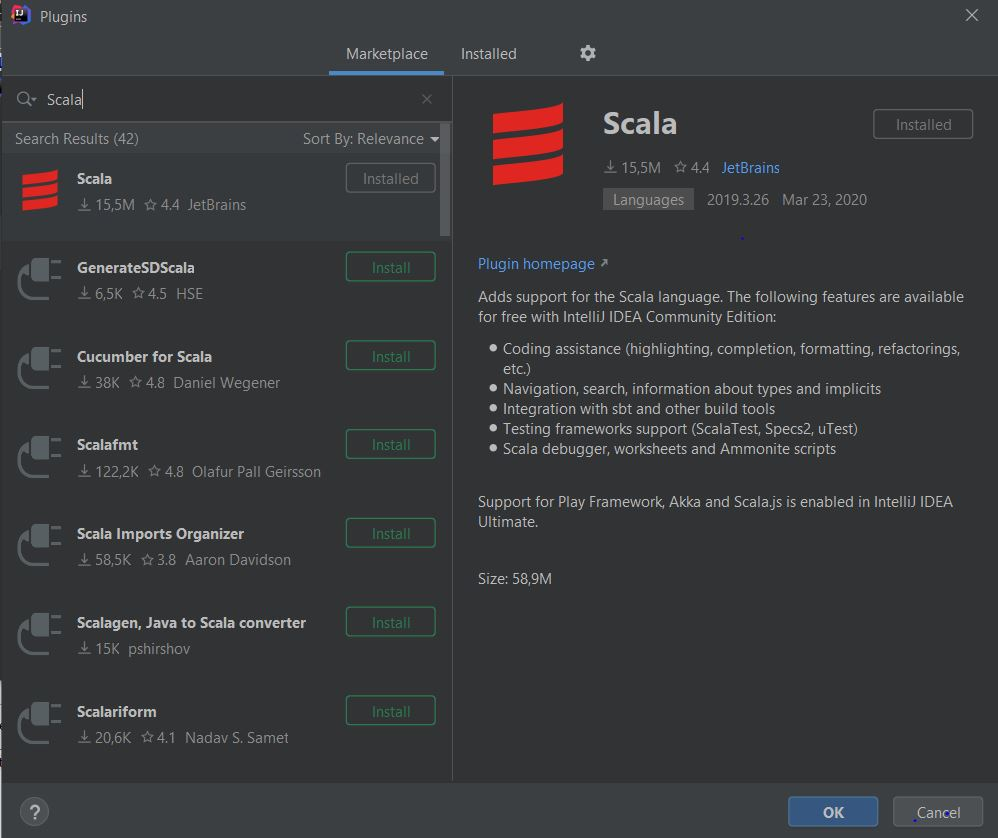
\includegraphics[scale=0.45]{intelij_2}
	\caption{Plugins Scala}
	\label{fig:intelij_2}
\end{figure}

\item Klik tombol \textit{install}

\end{enumerate}

\newpage
\subsection{Membuat \textit{Project} Spark pada IntelIJ}
Untuk membuat program Spark, pertama-tam perlu membuat project Spark baru untuk merancang kelas-kelas yang dibutuhkan pada eksekusi Spark. Beberapa hal yang perlu diperhatikan adalah menggunakan versi Scala sbt, memilih versi sbt 1.3.9, memilih versi Scala 2.11.12, dan melakukan \textit{import libraryDependencies} Spark sesuai kebutuhan.\\

\noindent Berikut adalah tahapan pembuatan \textit{project} Spark pada IntelIJ:

\begin{enumerate}
\item Memilih menu \textit{Create New Project}

\item Menggunakan bahasa pemrograman Scala berbasis sbt seperti Gambar \ref{fig:proyeksparksederhana1}.
\begin{figure}[H]
	\centering
	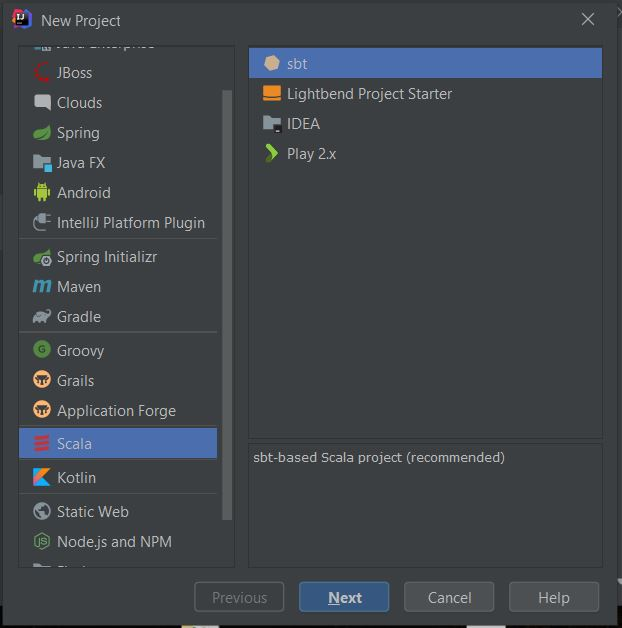
\includegraphics[scale=0.58]{proyeksparksederhana1.JPG}
	\caption{Memilih Bahasa Scala Berbasis sbt}
	\label{fig:proyeksparksederhana1}
\end{figure}

\item Melakukan konfigurasi pada project Spark baru seperti Gambar \ref{fig:proyeksparksederhana2}.
\begin{figure}[H]
	\centering
	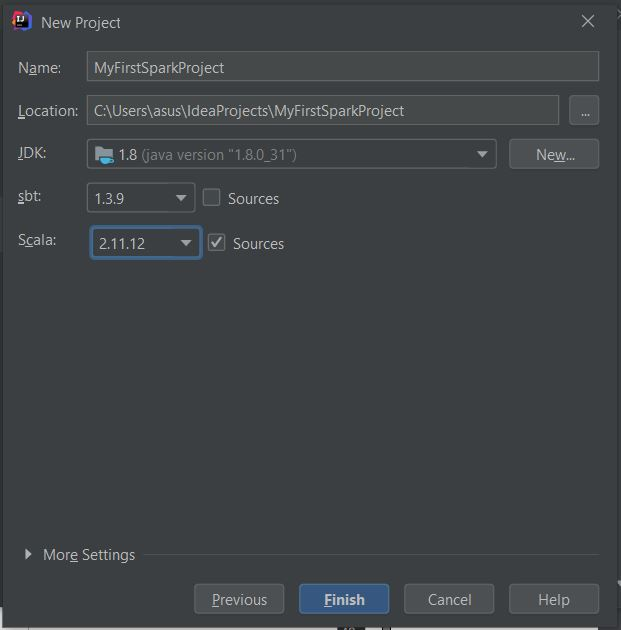
\includegraphics[scale=0.58]{proyeksparksederhana2.JPG}
	\caption{Melakukan Konfigurasi Project Spark}
	\label{fig:proyeksparksederhana2}
\end{figure}

\item Listing \ref{lst:build_sbt} adalah perintah \textit{import libraryDependencies} pada \textit{file} \path{build.sbt} \\ 
Contoh: spark-core, spark-sql, spark-mllib.
\begin{lstlisting}[basicstyle=\ttfamily, frame=single,
	columns=fullflexible, keepspaces=true, breaklines=true, label=lst:build_sbt, caption=Melakukan Import Library Spark]
name := "NamaProject"
version := "0.1"
scalaVersion := "2.11.12"
// https://mvnrepository.com/artifact/org.apache.spark/spark-core
libraryDependencies += "org.apache.spark" %% "spark-core" % "2.2.0"
// https://mvnrepository.com/artifact/org.apache.spark/spark-sql
libraryDependencies += "org.apache.spark" %% "spark-sql" % "2.4.0"
// https://mvnrepository.com/artifact/org.apache.spark/spark-mllib
libraryDependencies += "org.apache.spark" %% "spark-mllib" % "2.4.3"

\end{lstlisting}

\item Menambahkan \textit{Scala class} pada \path{src/main/scala} seperti Gambar \ref{fig:proyeksparksederhana5}.  
\begin{figure}[H]
	\centering
	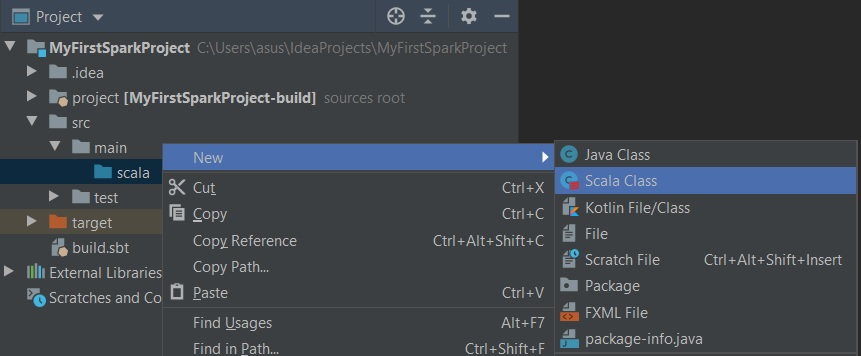
\includegraphics[scale=0.7]{proyeksparksederhana5.JPG}
	\caption{Menambahkan Scala Class pada Project Spark}
	\label{fig:proyeksparksederhana5}
\end{figure}

\item Memilih tipe \textit{Scala class} sebagai \textit{Object} seperti Gambar \ref{fig:proyeksparksederhana6}.
\begin{figure}[H]
	\centering
	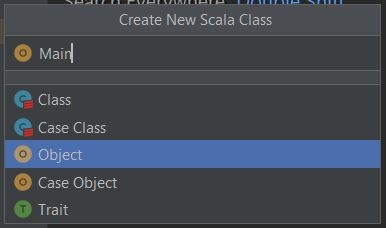
\includegraphics[scale=0.8]{proyeksparksederhana6.JPG} 
	\caption{Memilih Tipe Object pada Scala Class}
	\label{fig:proyeksparksederhana6}
\end{figure}

\item Listing \ref{lst:mainmethod} adalah perintah untuk menambahkan \textit{main method} pada \textit{Scala class}.
\begin{lstlisting}[basicstyle=\ttfamily, frame=single,
	columns=fullflexible, keepspaces=true, breaklines=true, label=lst:mainmethod, caption=Menambahkan Main method pada Scala Class]
object Main {
  def main(args: Array[String]) {
  	 //statement		
  }
}
\end{lstlisting}



\end{enumerate}

\subsection{Membuat \textit{File} JAR pada Command Prompt}
Sebelum menjalankan program Spark pada Hadoop Cluster, program Spark yang sudah jadi harus dibuat menjadi file JAR terlebih dahulu. Hal ini disebabkan karena perintah Spark hanya menerima input berupa kode program dalam format (.jar).\\

\noindent Berikut adalah tahapan untuk membuat File JAR:
\begin{enumerate}
\item Membuka folder pengerjaan \textit{project} Spark \path{\IdeaProjects\NamaProject}
\item Membuka command prompt pada folder \textit{project}.
\item Mengeksekusi perintah \textsf{sbt package} pada command prompt
\item Menunggu proses pembuatan file JAR oleh sistem, apabila terminal tidak menampilkan pesan \textit{error} maka file JAR telah berhasil dibuat dan tersimpan pada folder tertentu.
\item File JAR yang telah dibuat akan tersimpan pada \path{NamaProject\target\scala-2.11} 
\end{enumerate}

\subsection{Menjalankan Program Spark pada Komputer Lokal}
Apabila ukuran data input eksperimen kecil, maka program Spark dapat dijalankan pada komputer lokal menggunakan perintah dari Command Prompt. Waktu komputasi pada komputer lokal akan jauh lebih lama dibandingkan dijalankan pada server Hadoop Cluster. \\

\noindent Berikut adalah tahapan menjalankan program Spark pada komputer lokal:
\begin{enumerate}
\item Membuka \textit{command prompt} pada komputer lokal.
\item Menjalankan perintah eksekusi Spark sebagai berikut \textsf{spark-submit --class NamaMainClass --master local[*] \path{lokasi_jar\nama_jar.jar}} pada command prompt
\item Menunggu proses eksekusi file JAR oleh komputer lokal, apabila terminal tidak menampilkan pesan error maka program Spark berhasil dijalankan dengan baik.
\item Output yang dihasilkan oleh program Spark akan ditampilkan pada terminal \textit{command prompt}.
\end{enumerate}

\subsection{Menjalankan Program Spark pada Hadoop Cluster}
Karena ukuran data input eksperimen terbilang besar yaitu mencapai 1GB, maka akan lebih efektif apabila komputasi dilakukan secara paralel melalui Hadoop cluster. Hadoop cluster terdiri dari beberapa perangkat komputer yang dapat saling bekerja sama, sehingga proses komputasi dapat dilakukan lebih cepat.\\

\noindent Berikut adalah tahapan menjalankan program Spark pada Hadoop cluster:
\begin{enumerate}
\item Membuka \textit{command prompt} pada komputer lokal.
\item Menyambungkan jaringan komputer lokal dengan server Hadoop cluster menggunakan perintah \textsf{ssh hduser@10.100.69.101} pada command prompt.
\item Melakukan \textit{upload file} JAR dari komputer lokal ke folder Hadoop cluster menggunakan perintah \textsf{scp \path{nama_jar.jar} hduser
$@$10.100.69.101:\path{nama_folder}} pada command prompt.
\item Menjalankan perintah eksekusi Spark sebagai berikut \textsf{spark-submit --class NamaMainClass --master yarn \path{lokasi_jar\nama_jar.jar}} pada command prompt
\item Menunggu proses eksekusi \textit{file} JAR oleh Hadoop cluster, apabila terminal tidak menampilkan pesan error maka program Spark berhasil dijalankan dengan baik.
\end{enumerate}

\newpage
\section{Studi Kasus}
Untuk memahami implementasi algoritma anonimisasi pada Spark, maka dilakukan studi kasus terhadap fungsi Spark yang umum digunakan, seperti fungsi dasar pada Spark, fungsi dasar pada komponen Spark, dan fungsi dasar pada Spark MLlib. Bentuk dari studi kasus yang akan dilakukan adalah memberikan contoh kode program berikut penjelasan singkat mengenai tujuan pemanggilan fungsi, parameter input, dan contoh output yang dikeluarkan oleh fungsi tersebut.

\subsection{Eksperimen Scala}
Pada bagian \ref{sec:scala} telah dijelaskan tujuan dari penggunaan bahasa Scala. Scala digunakan pada penelitian ini karena sintaks yang sederhana untuk mengimplementasi beberapa baris kode pada bahasa pemrograman Java. Berikut adalah beberapa contoh ekperimen yang dilakukan pada bahasa Scala.

\subsubsection{Menentukan Jenis Variabel pada Scala}
Scala memiliki dua jenis varibel yaitu \textit{immutable} variabel dan mutable variabel. \textit{Immutable} variabel adalah variabel yang nilainya tidak dapat diubah, sedangkan \textit{mutable} variabel adalah variabel yang nilainya dapat diubah. Implementasi \textit{immutable} dan \textit{mutable} memiliki implementasi sintaks yang berbeda. \textit{Immutable} variabel menggunakan sintaks val, sedangkan \textit{mutable} variabel menggunakan sintaks var. Kode program dapat dilihat pada Listing \ref{lst:jenis_variabel} mengenai jenis variabel pada Scala.

\begin{lstlisting}[basicstyle=\ttfamily, frame=single,
	columns=fullflexible, keepspaces=true, breaklines=true, label=lst:jenis_variabel, caption=Menentukan Jenis Variabel pada Scala]
	
// Immutable Variabel
val donutsToBuy: Int = 5
donutsToBuy = 10

// Mutable Variabel
var favoriteDonut: String = "Glazed Donut"
favoriteDonut = "Vanilla Donut"


\end{lstlisting}

\subsubsection{Menentukan Jenis Tipe Data pada Scala}
Scala memiliki jenis tipe data yang mirip dengan tipe data pada bahasa pemrograman Java. Scala dapat menangani tipe data \textit{Int, Long, Short, Double, Float, String, Byte, Char} dan \textit{Unit}. Kode program dapat dilihat pada Listing \ref{lst:jenis_tipe_data} mengenai jenis tipe data pada Scala.

\begin{lstlisting}[basicstyle=\ttfamily, frame=single,
	columns=fullflexible, keepspaces=true, breaklines=true, label=lst:jenis_tipe_data, caption=Menentukan Jenis Tipe Data pada Scala]
	
val donutsBought: Int = 5
val bigNumberOfDonuts: Long = 10000000
val smallNumberOfDonuts: Short = 1
val priceOfDonut: Double = 2.50
val donutPrice: Float = 2.50f
val donutStoreName: String = "allaboutscala Donut Store"
val donutByte: Byte = 0xa
val donutFirstLetter: Char = 'D'
val nothing: Unit = ()

\end{lstlisting}

\newpage
\subsubsection{Menentukan Struktur Data pada Scala}
Scala memiliki dua jenis struktur data yaitu \textit{immutable} dan \textit{mutable collection}. \textit{Immutable collection} adalah struktur data yang nilainya tidak dapat diubah, sedangkan \textit{mutable collection} adalah struktur data yang nilainya dapat diubah. Implementasi \textit{immutable} dan \textit{mutable collection} memiliki jenis struktur data yang berbeda satu sama lain. Kode program dapat dilihat pada Listing \ref{lst:immutable_collection} mengenai \textit{immutable collection} pada Scala dan Listing \ref{lst:mutable_collection} mengenai \textit{mutable collection} pada Scala.

\begin{lstlisting}[basicstyle=\ttfamily, frame=single,
	columns=fullflexible, keepspaces=true, breaklines=true, label=lst:immutable_collection, caption=Membuat immutable collection pada Scala]
	
// List
val list1: List[String] = List("Plain Donut","Strawberry Donut","Chocolate Donut")
println(s"Elements of list1 = $list1")

// Map
val map1: Map[String, String] = Map(("PD","Plain Donut"),("SD","Strawberry Donut"),("CD","Chocolate Donut"))
println(s"Elements of map1 = $map1")

\end{lstlisting}

\begin{lstlisting}[basicstyle=\ttfamily, frame=single,
	columns=fullflexible, keepspaces=true, breaklines=true, label=lst:mutable_collection, caption=Membuat mutable collection pada Scala]
	
// Array
val array1: Array[String] = Array("Plain Donut","Strawberry Donut","Chocolate Donut")
println(s"Elements of array1 = ${array1.mkString(", ")}")

// Map
val map1: Map[String, String] = Map(("PD","Plain Donut"),("SD","Strawberry Donut"),("CD","Chocolate Donut"))
println(s"Elements of map1 = $map1")

\end{lstlisting}

\subsubsection{Membuat Kelas pada Scala}
Kelas pada Scala memiliki fungsi kelas yang sama pada Java yaitu untuk menyimpan variabel dan method. Kode program dapat dilihat pada Listing \ref{lst:class_scala} mengenai cara membuat kelas pada Scala.

\begin{lstlisting}[basicstyle=\ttfamily, frame=single,
	columns=fullflexible, keepspaces=true, breaklines=true, label=lst:class_scala, caption=Membuat Kelas Object pada Scala]
class AreaOfRectangle 
{ 
    var length = 20;  // Variables 
    var height = 40; 
      
    def area()  // Method which gives the area of the rectangle 
    { 
        var ar = length * height; 
        println("Area of the rectangle is :" + ar); 
    } 
} 
\end{lstlisting}

\subsubsection{Membuat \textit{Singleton Object} pada Scala}
Scala tidak memiliki variabel statik seperti pada Java, sehingga fungsinya digantikan oleh {\it singleton object}. {\it Singleton object} adalah objek yang mendefinisikan method main dari kelas-kelas pada Scala. Kode program dapat dilihat pada Listing \ref{lst:object_scala} mengenai cara membuat \textit{singletion object} pada Scala.

\begin{lstlisting}[basicstyle=\ttfamily, frame=single,
	columns=fullflexible, keepspaces=true, breaklines=true, label=lst:object_scala, caption=Membuat Kelas Object pada Scala]
object Main 
{ 
    def main(args: Array[String])  
    { 
        // Creating object of AreaOfRectangle class 
        var obj = new AreaOfRectangle(); 
        obj.area(); 
    } 
} 
\end{lstlisting}

\subsubsection{Membuat Fungsi Sederhana pada Scala}
Scala menggunakan fungsi untuk menempatkan kode program berdasarkan tujuan masing-masing. Perlu diperhatikan bahwa hasil akhir dari fungsi langsung dikembalikan tanpa memanggil perintah \textit{return}, seperti pada Java. Kode program dapat dilihat pada Listing \ref{lst:fungsi_sederhana} mengenai pembuatan fungsi pada Scala.

\begin{lstlisting}[basicstyle=\ttfamily, frame=single,
	columns=fullflexible, keepspaces=true, breaklines=true, label=lst:fungsi_sederhana, caption=Membuat Fungsi Sedehana pada Scala]
def calculateDonutCost(donutName: String, quantity: Int): Double = {
  println(s"Calculating cost for $donutName, quantity = $quantity")

  // make some calculations ...
  2.50 * quantity
}
\end{lstlisting}

\subsubsection{Membuat Fungsi Percabangan}
Scala memiliki jenis implementasi percabangan yang sama dengan Java. Percabangan digunakan untuk melakukan eksekusi pada baris \textit{statement} yang sesuai berdasarkan kondisi tertentu. Kode program dapat dilihat pada Listing \ref{lst:percabangan} mengenai percabangan pada Scala.

\begin{lstlisting}[basicstyle=\ttfamily, frame=single,
	columns=fullflexible, keepspaces=true, breaklines=true, label=lst:percabangan, caption=Membuat Fungsi Percabangan pada Scala]
# If-Else statement
if(numberOfPeople > 10) { 
  println(s"Number of donuts to buy = ${numberOfPeople * donutsPerPerson}")
}
else if (numberOfPeople == 0) {
  println("Number of people is zero.")
  println("No need to buy donuts.")
} 
else {
  println(s"Number of donuts to buy = $defaultDonutsToBuy")
}
\end{lstlisting}

\subsubsection{Membuat Fungsi Perulangan pada Scala}
Scala memiliki jenis implementasi perulangan yang sama dengan Java. Perulangan digunakan untuk mengulangi eksekusi pada baris statement yang sama berdasarkan kondisi tertentu. Kode program dapat dilihat pada Listing \ref{lst:perulangan} mengenai perulangan pada Scala.

\begin{lstlisting}[basicstyle=\ttfamily, frame=single,
	columns=fullflexible, keepspaces=true, breaklines=true, label=lst:perulangan, caption=Membuat Fungsi Perulangan pada Scala]
# For loop
for(numberOfDonuts <- 1 to 5){
  println(s"Number of donuts to buy = $numberOfDonuts")
}

# While loop
while (numberOfDonutsToBake > 0) {
  println(s"Remaining donuts to be baked = $numberOfDonutsToBake")
  numberOfDonutsToBake -= 1
}

# Do-while loop
do {
  numberOfDonutsBaked += 1
  println(s"Number of donuts baked = $numberOfDonutsBaked")
} 
while (numberOfDonutsBaked < 5)
\end{lstlisting}



\subsection{Eksperimen Spark}
Spark adalah teknologi yang digunakan untuk mengolah \textit{big data} berdasarkan konsep dari bagian \ref{sec:konsep_spark}. Spark membagi satu pekerjaan pada masing-masing \textit{Worker Node} seperti pada bagian \ref{sec:arsitektur_spark}. Oleh karena itu Spark memecah data partisi data agar data yang besar dapat distribusikan ke masing-masing komputer. Berikut adalah beberapa fungsi dasar Spark untuk mengolah partisi data.

\subsubsection{Melakukan Konfigurasi Spark}
Berikut adalah tahapan konfigurasi Spark pada Main Class:
\begin{itemize}
\item Membuat objek SparkConf untuk inisialisasi project Spark
\item Menetapkan jumlah \textit{core} CPU yang bekerja pada perintah setMaster()
\item Menetapkan nama program Spark pada perintah setAppName()
\item Membuat objek SparkContext untuk membuat RDD.

\end{itemize}

\begin{lstlisting}[basicstyle=\ttfamily, frame=single,
	columns=fullflexible, keepspaces=true, breaklines=true, label=ls_kepatuhan_1_1_1_logo_sharif_judge, caption=Konfigurasi Spark]
	
val conf = new SparkConf()
conf.setMaster("local[2]")
conf.setAppName("Tutorial Spark")
val sc = new SparkContext(conf)


\end{lstlisting}
  
\newpage
\subsubsection{Membuat RDD}
Pada bagian \ref{sec:rdd}, sudah dijelaskan konsep RDD. Pada bagian ini, akan dilakukan eksperimen mengenai jenis-jenis cara untuk membuat RDD pada Spark.\\

\noindent Berikut adalah beberapa cara untuk membuat RDD:
\begin{itemize}
\item Membaca data eksternal pada Spark sebagai RDD
\item Membuat RDD dari struktur data \textit{List}
\item Merubah Dataframe menjadi RDD
\end{itemize}

\begin{lstlisting}[basicstyle=\ttfamily, frame=single,
	columns=fullflexible, keepspaces=true, breaklines=true, label=ls_kepatuhan_1_1_1_logo_sharif_judge, caption=Cara Pembuatan RDD]
	
# 1. Membaca data eksternal pada Spark sebagai RD
rdd = sc.textFile("path")

# 2. Membuat RDD dari struktur data list
rdd = sc.parallelize(["id","name","3","5"])

# 3. Merubah Dataframe menjadi RDD
rdd = df.rdd

\end{lstlisting}

\subsubsection{Membuat Dataframe}
Pada bagian \ref{sec:dataframe}, sudah dijelaskan konsep \textit{DataFrame}. Pada bagian ini, akan dilakukan eksperimen mengenai jenis-jenis cara untuk membuat \textit{DataFrame} pada Spark.\\

\noindent Berikut adalah beberapa cara untuk membuat \textit{DataFrame}:
\begin{itemize}
\item Membaca data eksternal sebagai \textit{DataFrame}
\item Mengubah RDD menjadi \textit{DataFrame} dengan nama kolom
\item Mengubah RDD menjadi \textit{DataFrame} dengan skema
\end{itemize}
\begin{lstlisting}[basicstyle=\ttfamily, frame=single,
	columns=fullflexible, keepspaces=true, breaklines=true, label=ls_kepatuhan_1_1_1_logo_sharif_judge, caption=Cara Pembuatan Dataframe]
	
# 1. Membaca data eksternal sebagai Dataframe
#  header and schema are optional
df = sqlContext.read.csv("path", header = True/False, schema=df_schema)

# 2.1 Mengubah RDD menjadi Dataframe dengan nama kolom
df = spark.createDataFrame(rdd,["name","age"])

# 2.2 Mengubah RDD menjadi Dataframe dengan skema
from pyspark.sql.types import *
df_schema = StructType([
...    StructField("name", StringType(), True),
...    StructField("age", IntegerType(), True)])
df = spark.createDataFrame(rdd,df_schema)

\end{lstlisting}

\newpage
\subsubsection{Memanggil Fungsi \textit{Transformation}}
\noindent Pada bagian \ref{sec:fungsi_rdd} dijelaskan jenis-jenis fungsi \textit{Transformation} pada RDD. Listing \ref{lst:transformation} adalah contoh penerapan jenis-jenis fungsi \textit{Tranformation} pada Spark, berikut adalah penjelasan singkat dari masing-masing fungsi:
\begin{itemize}
\item select(): menampilkan isi RDD berdasarkan nama variabel yang menyimpan RDD.
\item filter()/where(): menyeleksi isi RDD berdasarkan kondisi tertentu
\item sort()/orderBy(): mengurutkan isi RDD berdasarkan keterurutan atribut tertentu
\item groupBy() dan agg(): mengelompokan isi RDD dan melakukan agregasi.
\item join(): menggabungkan dua RDD yang berbeda berdasarkan kesamaan nilai atribut.
\end{itemize}

\begin{lstlisting}[basicstyle=\ttfamily, frame=single,
	columns=fullflexible, keepspaces=true, breaklines=true, label=lst:transformation, caption=Contoh Fungsi Transformation]
	
# 1. select
df.select(df.name)
df.select("name")

# 2. filter/where
df.filter(df.age>20)
df.filter("age>20")
df.where("age>20")
df.where(df.age>20)
 
# 3. sort/orderBy 
df.sort("age",ascending=False)
df.orderBy(df.age.desct())
 
# 4. groupBy dan agg
df.groupBy("gender").agg(count("name"),avg("age"))

# 5. join
df1.join(df.2, (df1.x1 == df2.x1) & (df1.x2 == df2.x2),'left')

\end{lstlisting}

\subsubsection{Memanggil Fungsi \textit{Action}}
\noindent Pada bagian \ref{sec:fungsi_rdd} dijelaskan jenis-jenis fungsi \textit{Action} pada RDD. Listing \ref{lst:action} adalah contoh penerapan jenis-jenis fungsi \textit{Action} pada Spark, berikut adalah penjelasan singkat dari masing-masing fungsi:
\begin{itemize}
\item show(): menampilkan n baris pertama dari \textit{DataFrame} atau RDD
\item take(): menampilkan beberapa baris dari \textit{DataFrame} atau RDD
\item collect(): mengumpulkan seluruhdata dari \textit{DataFrame} atau RDD 
\item count(): menghitung jumlah baris
\item printSchema(): menampilkan nama kolom dan tipe data
\end{itemize}

\begin{lstlisting}[basicstyle=\ttfamily, frame=single,
	columns=fullflexible, keepspaces=true, breaklines=true, label=lst:action, caption=Contoh Fungsi Action]
# 1. show()
df.show(5)

# 2. take()
df.take(5)

# 3. collect()
df.collect()

# 4. count()
df.count()

# 6. printSchema()
df.printSchema()

# 7. transformation, action
df1.filter("age>10").join(df2,df1.x==df2.y).sort("age").show()


\end{lstlisting}

\subsubsection{Memanggil Fungsi RDD}
\noindent Listing \ref{lst:fungsi_rdd} adalah contoh penerapan jenis-jenis fungsi RDD pada Spark, berikut adalah penjelasan singkat dari masing-masing fungsi RDD:

\begin{itemize}
\item repartition(n): membagi RDD menjadi n buah partisi
\item cache(): menyimpan RDD pada penyimpanan memori.
\item persist(): menyimpan RDD pada penyimpanan memori atau disk.
\item unpersist(): menghapus RDD pada memori atau disk.
\item foreach(println): melakukan print seluruh baris data pada RDD
\item saveAsTextFile(path): menyimpan RDD pada sebuah file
\end{itemize}

\begin{lstlisting}[basicstyle=\ttfamily, frame=single,
	columns=fullflexible, keepspaces=true, breaklines=true, label=lst:fungsi_rdd, caption=Contoh Fungsi RDD]
rdd.repartition(4)
rdd.cache() 
rdd.persist() 
rdd.unpersist()
rdd.foreach(println)
rdd.saveAsTextFile(path)

\end{lstlisting}

\subsubsection{Membuat Variabel Global}
\noindent Listing \ref{lst:var_global} adalah perintah untuk membuat variabel global pada Spark.
\begin{lstlisting}[basicstyle=\ttfamily, frame=single,
	columns=fullflexible, keepspaces=true, breaklines=true, label=lst:var_global, caption=Membuat Variabel Global]
val broadcastVar = sc.broadcast(Array(1, 2, 3))
\end{lstlisting}	

\newpage
\subsection{Eksperimen Komponen Spark}
Pada bagian \ref{sec:komponen_spark} dijelaskan mengenai jenis-jenis komponen Spark dan tujuan penggunaannya. Pada bagian ini akan dilakukan eksperimen berdasarkan masing-masing jenis komponen Spark.

\subsubsection{Spark Core}
\noindent Berikut adalah langkah-langkah eksperimen dari Spark Core:
\begin{enumerate}

\item Listing \ref{lst:sparksession} adalah membuat perintah SparkSession untuk inisialisasi project Spark
\begin{lstlisting}[basicstyle=\ttfamily, frame=single,
	columns=fullflexible, keepspaces=true, breaklines=true, label=lst:sparksession, caption=Membuat SparkSession]

val spark: SparkSession = SparkSession.builder()
      .master("local[3]")
      .appName("SparkCoreAdults")
      .getOrCreate()	
      
\end{lstlisting}

\item Listing \ref{lst:partisiRDD} adalah melihat dan mengatur partisi RDD berdasarkan data input CSV 
\begin{lstlisting}[basicstyle=\ttfamily, frame=single,
	columns=fullflexible, keepspaces=true, breaklines=true, label=lst:partisiRDD, caption=Melihat dan Mengatur Partisi RDD]
	
val sc = spark.sparkContext

val rdd: RDD[String] = sc.textFile("input/adult100k.csv")
println("initial partition count:" + rdd.getNumPartitions)

val reparRdd = rdd.repartition(4)
println("re-partition count:" + reparRdd.getNumPartitions)	
	
\end{lstlisting}

\item Listing \ref{lst:transSparkCore} adalah membuat jenis-jenis fungsi \textit{transformation}.
\begin{lstlisting}[basicstyle=\ttfamily, frame=single,
	columns=fullflexible, keepspaces=true, breaklines=true, label=lst:transSparkCore, caption=Membuat Fungsi Transformation]
	
//Transformation - flatMap
val rdd2 = rdd.flatMap(f => f.split(","))
rdd2.foreach(f => println(f))

//Transformation - map
val rdd3: RDD[(String, Int)] = rdd2.map(key => (key, 1))
rdd3.foreach(println)

//Transformation - filter
val rdd4 = rdd3.filter(a => a._1.startsWith("State-gov"))
rdd4.foreach(println)

//Transformation - reduceByKey
val rdd5 = rdd3.reduceByKey((x,y)=> x + y)
rdd5.foreach(println)

//Transformation - sortByKey
val rdd6 = rdd5.map(a => (a._2, a._1)).sortByKey()
    
\end{lstlisting}

\newpage
\item Listing \ref{lst:actionSparkCore} adalah membuat jenis-jenis fungsi \textit{action}.
\begin{lstlisting}[basicstyle=\ttfamily, frame=single,
	columns=fullflexible, keepspaces=true, breaklines=true, label=lst:actionSparkCore, caption=Membuat Fungsi Action]

//Action - count
println("Count : " + rdd6.count())

//Action - first
val firstRec = rdd6.first()
println("First Record : " + firstRec._1 + "," + firstRec._2)

//Action - max
val datMax = rdd6.max()
println("Max Record : " + datMax._1 + "," + datMax._2)

//Action - reduce
val totalWordCount = rdd6.reduce((a, b) => (a._1 + b._1, a._2))
println("dataReduce Record : " + totalWordCount._1)

//Action - take
val data3 = rdd6.take(3)
data3.foreach(f => {
	println("data3 Key:" + f._1 + ", Value:" + f._2)
})

//Action - collect
val data = rdd6.collect()
data.foreach(f => {
	println("Key:" + f._1 + ", Value:" + f._2)
})

//Action - saveAsTextFile
rdd5.saveAsTextFile("c:/tmp/wordCount")
	
\end{lstlisting}

\end{enumerate}


\subsubsection{Spark SQL}
\noindent Berikut adalah langkah-langkah eksperimen dari Spark Core:
\begin{enumerate}

\item Listing \ref{lst:sparksession_sql} adalah perintah untuk membuat SparkSession saat inisialisasi \textit{project} Spark
\begin{lstlisting}[basicstyle=\ttfamily, frame=single,
	columns=fullflexible, keepspaces=true, breaklines=true, label=lst:sparksession_sql, caption=Membuat Perintah SparkSession]
	
val spark = SparkSession
	.builder.master("local[*]")
	.appName("SparkSQL")
	.getOrCreate()	
	
\end{lstlisting}

\newpage
\item Listing \ref{lst:dataframe_sql} adalah perintah untuk membuat \textit{DataFrame} dari data input CSV.
\begin{lstlisting}[basicstyle=\ttfamily, frame=single,
	columns=fullflexible, keepspaces=true, breaklines=true, label=lst:dataframe_sql, caption=Membuat Dataframe]
	
val peopleDF = spark.read
	.format("csv")
	.option("header", "true")
	.option("delimiter", ",")
	.load("input/adult100k.csv")

peopleDF.printSchema()	
	
\end{lstlisting}

\item Listing \ref{lst:tabelsementara_sql} adalah perintah untuk membuat tabel sementara, melakukan kueri, dan menyimpan hasil kueri pada file CSV.
\begin{lstlisting}[basicstyle=\ttfamily, frame=single,
	columns=fullflexible, keepspaces=true, breaklines=true, label=lst:tabelsementara_sql, caption=Membuat Tabel Sementara]
	
// Query
peopleDF.createTempView("tAdults")
val query = spark.sql(
	"SELECT workclass,count(education) as count_people"+
	"FROM tAdults " +
	"WHERE lower(education) == 'bachelors'" +
	"GROUP BY workclass " +
	"ORDER BY count_people DESC " +
	"LIMIT 10"
)	
query.write.csv("C:/Users/asus/Desktop/resultquery1.csv")
	
\end{lstlisting}

\item Listing \ref{lst:statistik_sql} adalah perintah untuk mencari nilai statistik seperti jumlah data, \textit{mean}, standar deviasi, nilai minimum dan maksimum.
\begin{lstlisting}[basicstyle=\ttfamily, frame=single,
	columns=fullflexible, keepspaces=true, breaklines=true, label=lst:statistik_sql, caption=Mencari Nilai Statistik]
	
// Statistika: count, mean, stddev, min, max
peopleDF.describe().show()
    
\end{lstlisting}

\item Listing \ref{lst:median_sql} adalah perintah untuk mencari nilai \textit{median}.
\begin{lstlisting}[basicstyle=\ttfamily, frame=single,
	columns=fullflexible, keepspaces=true, breaklines=true, label=lst:median_sql, caption=Mencari Nilai Median]
	
// Median
val median = spark.sql(
	"SELECT percentile_approx(age, 0.5) as Median " +
	"FROM tAdults"
).show()

\end{lstlisting}

\newpage
\item Listing \ref{lst:modus_sql} adalah perintah untuk mencari nilai \textit{modus}.
\begin{lstlisting}[basicstyle=\ttfamily, frame=single,
	columns=fullflexible, keepspaces=true, breaklines=true, label=lst:modus_sql, caption=Mencari Nilai Modus]
	
// Modus
val modus = spark.sql( 
 	"SELECT age as Modus " +
	"FROM tAdults " +
	"GROUP BY age " +
	"ORDER BY COUNT(age) DESC " +
	"LIMIT 1"
).show()

\end{lstlisting}

\end{enumerate}


\subsubsection{Spark MLlib}
\noindent Berikut adalah langkah-langkah eksperimen dari Spark Core:
\begin{enumerate}

\item Listing \ref{lst:sparksession_mllib} adalah perintah untuk membuat SparkSession saat inisialisasi \textit{project} Spark
\begin{lstlisting}[basicstyle=\ttfamily, frame=single,
	columns=fullflexible, keepspaces=true, breaklines=true, label=lst:sparksession_mllib, caption=Membuat Perintah SparkSession]
	
val spark = SparkSession
      .builder.master("local[*]")
      .appName("SparkMLlib")
      .getOrCreate()
	
\end{lstlisting}

\item Listing \ref{lst:skema_mllib} adalah perintah untuk membuat skema untuk \textit{DataFrame}. 
\begin{lstlisting}[basicstyle=\ttfamily, frame=single,
	columns=fullflexible, keepspaces=true, breaklines=true, label=lst:skema_mllib, caption=Membuat Skema Dataframe]
	
val schema = StructType(
      List(
        StructField("age", IntegerType, true),
        StructField("workclass", StringType, true),
        StructField("fnlwgt", IntegerType, true),
        StructField("education", StringType, true),
        StructField("education-num", IntegerType, true),
        StructField("marital-status", StringType, true),
        StructField("occupation", StringType, true),
        StructField("relationship", StringType, true),
        StructField("race", StringType, true),
        StructField("sex", StringType, true),
        StructField("capital-gain", IntegerType, true),
        StructField("capital-loss", IntegerType, true),
        StructField("hours-per-week", IntegerType, true),
        StructField("native-country", StringType, true),
        StructField("salary", StringType, true)
      )
    )
    	
\end{lstlisting}

\item Listing \ref{lst:skemacsv_mllib} adalah perintah untuk mengubah data input CSV menjadi \textit{DataFrame} berdasarkan skema.
\begin{lstlisting}[basicstyle=\ttfamily, frame=single,
	columns=fullflexible, keepspaces=true, breaklines=true, label=lst:skemacsv_mllib, caption=Mengubah CSV Menjadi Dataframe]
val adult100k_df = spark.read
      .format("csv")
      .option("header", "false")
      .option("delimiter", ",")
      .schema(schema)
      .load("input/adult100k.csv")

adult100k_df.show()	
\end{lstlisting}

\item Listing \ref{lst:kolomindex_mllib} adalah perintah untuk menggunakan fungsi \textit{stringIndexer} untuk membuat kolom indeks dan fungsi \textit{oneHotEncoder} untuk membuat kolom vektor.
\begin{lstlisting}[basicstyle=\ttfamily, frame=single,
	columns=fullflexible, keepspaces=true, breaklines=true, label=lst:kolomindex_mllib, caption=Membuat Kolom Index]
// Create vector based on stringIndexer and oneHotEncoder
val cols = adult100k_df.columns
val encodedFeatures = cols.flatMap{columnName =>
	val stringIndexer = new StringIndexer()
		.setInputCol(columnName)
		.setOutputCol(columnName + "_Index")
	val oneHotEncoder = new OneHotEncoderEstimator()
		.setInputCols(Array(columnName + "_Index"))
		.setOutputCols(Array(columnName + "_vec"))
		.setDropLast(false)
	Array(stringIndexer.setHandleInvalid("keep"),oneHotEncoder)
}	
\end{lstlisting}

\item Listing \ref{lst:kolomvektor_mllib} adalah perintah untuk menambahkan kolom vektor dan kolom indeks pada \textit{DataFrame}.
\begin{lstlisting}[basicstyle=\ttfamily, frame=single,
	columns=fullflexible, keepspaces=true, breaklines=true, label=lst:kolomvektor_mllib, caption=Membuat Kolom Vektor]
// Pipeline
val pipeline = new Pipeline().setStages(encodedFeatures)
val indexer_model = pipeline.fit(adult100k_df)
\end{lstlisting}

\item Listing \ref{lst:jenisvektor_mllib} adalah perintah untuk memilih jenis implementasi vektor yang akan digunakan.
\begin{lstlisting}[basicstyle=\ttfamily, frame=single,
	columns=fullflexible, keepspaces=true, breaklines=true, label=lst:jenisvektor_mllib, caption=Memilih Jenis Vektor]
// Sparse Vector
val df_transformed = indexer_model.transform(adult100k_df)
df_transformed.show()

// Dense Vector
val sparseToDense = udf((v: Vector) => v.toDense)
val df_denseVectors = df_transformed
		.withColumn("dense_workclass_vec",
		sparseToDense(df_transformed("workclass_vec")))
df_denseVectors.show()	
\end{lstlisting}

\newpage
\item Listing \ref{lst:feature_mllib} adalah perintah untuk membuat vektor fitur dari setiap baris data pada \textit{DataFrame}.
\begin{lstlisting}[basicstyle=\ttfamily, frame=single,
	columns=fullflexible, keepspaces=true, breaklines=true, label=lst:feature_mllib, caption=Membuat Vektor Fitur]
// Final Result: Feature Vector
val vecFeatures = df_transformed.columns.filter(_.contains("vec"))
val vectorAssembler = new VectorAssembler()
		.setInputCols(vecFeatures)
		.setOutputCol("features")
val pipelineVectorAssembler = new Pipeline()
		.setStages(Array(vectorAssembler))
val result_df = pipelineVectorAssembler
		.fit(df_transformed)
		.transform(df_transformed)
result_df.show()
\end{lstlisting}

\end{enumerate}


\subsection{Eksperimen Spark MLIB}
Pada bagian \ref{sec:konsep_spark_mllib} telah dijelaskan mengenai konsep dan contoh pemodelan pada Spark MLlib. Pada penelitian ini akan digunakan pemodelan \textit{Naive Bayes} untuk permasalahan klasifikasi pada bagian \ref{sec:naive_bayes} dan \textit{k-means} untuk permasalahan clustering pada bagian \ref{sec:k_means}.

\subsubsection{\textit{Naive Bayes}}
\noindent Pada bagian \ref{sec:naivebayes_mllib} menjelaskan parameter pemodelan \textit{Naive Bayes} pada Spark MLlib. Berikut adalah tahapan eksperimen pada Listing \ref{lst:naivebayes_mllib} untuk pemodelan \textit{Naive Bayes}:
\begin{enumerate}
\item Membagi data input CSV menjadi training data dan test data.
\item Melakukan pelatihan data pada pemodelan Naive Bayes.
\item Mengembalikan hasil klasifikasi dalam bentuk tabel.
\item Menghitung akurasi dari klasifikasi label kelas.
\end{enumerate}	

\begin{lstlisting}[basicstyle=\ttfamily, frame=single,
	columns=fullflexible, keepspaces=true, breaklines=true, label=lst:naivebayes_mllib, caption=Eksperimen Naive Bayes Spark MLlib]
// Split data into training (70%) and test (30%).
val Array(training, test) = result_df.randomSplit(Array(0.7, 0.3))

// Naive Bayes
val model = new NaiveBayes().setModelType("multinomial")
			.setLabelCol("workclass_Index").fit(training)
			
// Predict model
val predictions = model.transform(test)
predictions.show()

// Accuracy
val evaluator = new MulticlassClassificationEvaluator()
	.setLabelCol("workclass_Index")
	.setPredictionCol("prediction")
	.setMetricName("accuracy")
val accuracy = evaluator.evaluate(predictions)

\end{lstlisting}



\newpage
\noindent Dataset yang dipakai untuk eksperimen \textit{naive bayes} ini adalah sampel data dari dataset Adult yang sudah dijelaskan pada bagian. Data ini berjumlah 100.000 baris data dengan ukuran 11.000 KB. Dataset ini akan dibagi menjadi data test dan data training. Jumlah data test adalah 30.000 baris data, sedangkan jumlah data training adalah 70.000 data. Jumlah data training lebih banyak karena akan dipakai untuk pelatihan model \textit{naive bayes}.

\begin{figure}[H]
	\centering
	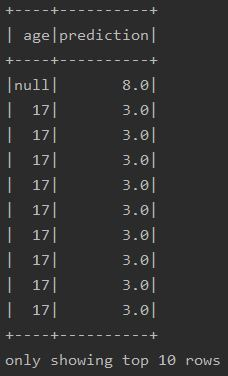
\includegraphics[scale=0.65]{mllib_naivebayes}
	\caption{Hasil Naive Bayes Spark MLlib}
	\label{fig:mllib_naivebayes}
\end{figure}

\noindent Hasil pemodelan \textit{naive bayes} dari eksperimen ini adalah label data. Cluster ini terbentuk berdasarkan distance terdekat antara anggota data dengan titik centroid pada cluster tersebut. Sehingga data-data yang tergabung pada sebuah cluster, sudah dipastikan bahwa data-data tersebut lebih dekat dengan titik centroid pada cluster tersebut dibanding dengan titik centroid pada cluster lainnya. Gambar \ref{fig:mllib_naivebayes} menunjukan bahwa data dengan nilai umur yang sama (\textit{age} = 17) memiliki kelompok cluster yang sama (\textit{prediction} = 3.0).


\subsubsection{\textit{K-Means}}
\noindent Pada bagian \ref{sec:kmeans_mllib} menjelaskan parameter pemodelan \textit{k-means} pada Spark MLlib. Berikut adalah tahapan eksperimen pada Listing \ref{lst:kmeans_mllib} untuk pemodelan \textit{k-means}:

\begin{enumerate}
\item Membuat model \textit{k-means} menggunakan Spark MLlib
\item Menentukan jumlah cluster (k) untuk pemodelan \textit{k-means}.
\item Melakukan pelatihan data pada pemodelan \textit{k-means}.
\item Mencari nilai \textit{centroid} dari masing-masing \textit{cluster}.
\item Mengembalikan hasil \textit{clustering} dalam bentuk tabel.
\end{enumerate}	

\begin{lstlisting}[basicstyle=\ttfamily, frame=single,
	columns=fullflexible, keepspaces=true, breaklines=true, label=lst:kmeans_mllib, caption=Eksperimen K-Means Spark MLlib]
// KMeans with 8 clusters
val kmeans = new KMeans()
      .setK(8)
      .setFeaturesCol("features")
      .setPredictionCol("prediction")
val kmeansModel = kmeans.fit(result_df)
kmeansModel.clusterCenters.foreach(println)

// Predict model
val predictDf = kmeansModel.transform(result_df)
predictDf.show(10)

\end{lstlisting}

\noindent Dataset yang dipakai untuk eksperimen \textit{k-means} ini adalah sampel data dari dataset Adult yang sudah dijelaskan pada bagian. Data ini berjumlah 100.000 baris data dengan ukuran 11.000 KB. Batas maksimum iterasi untuk fungsi k-means telah diatur sedemikian rupa oleh library Spark MLlib itu sendiri, sehingga parameter ini tidak perlu lagi diset manual oleh pengguna. Jumlah cluster yang akan dibentuk pada eksperimen ini berjumlah 8 cluster. Jumlah cluster pada fungsi k-means nantinya dapat diatur kembali sesuai kebutuhan eksperimen.

\begin{figure}[H]
	\centering
	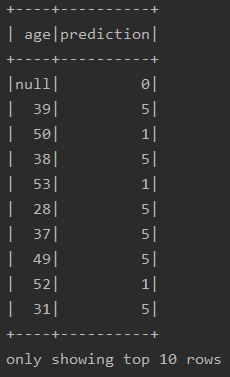
\includegraphics[scale=0.65]{mllib_kmeans}
	\caption{Hasil K-Means Spark MLlib}
	\label{fig:mllib_kmeans}
\end{figure}

\noindent Hasil pemodelan \textit{k-means} dari eksperimen ini adalah \textit{cluster} data. Cluster ini terbentuk berdasarkan distance terdekat antara anggota data dengan titik centroid pada cluster tersebut. Sehingga data-data yang tergabung pada sebuah cluster, sudah dipastikan bahwa data-data tersebut lebih dekat dengan titik centroid pada cluster tersebut dibanding dengan titik centroid pada cluster lainnya. Gambar \ref{fig:mllib_kmeans} menunjukan bahwa data dengan atribut (\textit{age} = 39) memiliki kelompok \textit{cluster} yang sama dengan dengan data lain dengan atribut (\textit{age} = 38), karena berada pada kelompok data yang sama dengan representasi nama kelompok (\textit{prediction} = 5).

\section{Gambaran Umum Perangkat Lunak}
Penelitian ini menghasilkan dua jenis perangkat lunak dengan tujuan yang berbeda satu sama lain, untuk menyelesaikan permasalahan penerapan algorima \textit{Greedy k-member clustering} pada lingkungan \textit{big data}. Berikut adalah deskripsi perangkat lunak yang akan dibuat:

\begin{enumerate}

\item Perangkat lunak dapat mengimplementasikan algoritma \textit{k-anonymity}. Algoritma \textit{k-anonymity} yang dimaksud adalah algoritma \textit{Greedy k-member clustering}. Masukan dari perangkat lunak ini adalah dataset \textit{Adult} dalam format file CSV, tabel atribut quasi-identifier (QID), dan parameter dari algoritma \textit{Greedy k-member clustering} yaitu nilai k dan objek \textit{Domain Generalization Hierarchy} (DGH). Keluaran dari perangkat lunak ini adalah hasil anonimisasi dari dataset \textit{Adult} yang disimpan dalam format \textit{file} CSV.

\item Perangkat lunak dapat membandingkan hasil anonimisasi algoritma \textit{k-anonymity} melalui metode \textit{data mining} yang telah disediakan. Metode \textit{data mining} yang akan disediakan adalah klasifikasi dengan pemodelan \textit{Naive Bayes} dan pengelompokan/\textit{clustering} dengan pemodelan \textit{k-means}. Masukan dari perangkat lunak ini adalah dataset \textit{Adult} dalam format \textit{file} CSV, baik dataset pernah dilakukan proses anonimisasi maupun dataset asli. Untuk pemodelan \textit{k-means} membutuhkan parameter tambahan seperti nilai k dan jenis atribut yang akan diprediksi nilainya. Sedangkan untuk pemodelan \textit{Naive Bayes} membutuhkan parameter tambahan seperti persentase antara \textit{training} dan \textit{testing} data, jenis atribut yang akan diprediksi nilainya. Keluaran dari perangkat lunak ini untuk pemodelan \textit{Naive Bayes} dan \textit{k-means} memiliki hasil yang sama, yaitu jenis nilai dari atribut yang telah dipilih dan jenis \textit{cluster}.

\end{enumerate}

\subsection{Diagram Aktifitas}
Penelitian ini memiliki dua jenis diagram aktivitas,  yaitu diagram aktivitas untuk perangkat lunak anonimisasi data dan diagram aktivitas untuk perangkat lunak analisis data. Tujuan dari membuat dua jenis perangkat lunak antara lain untuk memisahkan perangkat lunak dari fungsionalitas yang berbeda. Fungsionalitas tersebut antara lain melakukan proses anonimisasi data pada dataset dan membandingkan hasil antara dataset asli dengan dataset yang telah dilakukan proses anonimisasi untuk mencari tahu seberapa baik kinerja algoritma \textit{Greedy k-member clustering} untuk mendapatkan hasil yang informatif.

\subsubsection{Perangkat Lunak Anonimisasi Data}
Perangkat lunak ini bertujuan untuk melakukan proses anonimisasi pada dataset \textit{Adult} menggunakan algoritma \textit{k-anonymity}. Diagram aktifitas dapat dilihat pada Gambar \ref{fig:pl_anonimisasi}, berikut adalah tahapan yang terjadi pada perangkat lunak saat melakukan proses anonimisasi data:

\begin{enumerate}

\item Pengguna memberi masukan dalam format file CSV dan beberapa jenis atribut \textit{quasi-identifier} untuk menjadi tabel input pada proses anonimisasi.

\item Perangkat lunak menampilkan sebagian baris data dari tabel input karena baris data yang akan digunakan pada eksperimen akan berjumlah sangat banyak .

\item Pengguna akan meninjau ulang apakah jumlah kolom yang ditampilkan sudah sesuai dengan jumlah atribut \textit{quasi-identifier} yang akan dipakai.

\item Penggunakan memberikan parameter tambahan seperti rentang nilai k untuk menentukan jumlah anggota \textit{cluster} dan objek DGH untuk proses anonimisasi.

\item Perangkat lunak akan melakukan proses anonimisasi dengan bantuan Spark pada tabel input berdasarkan paramater tambahan yang diberikan sebelumnya. 

\item Perangkat lunak mengembalikan seluruh isi \textit{log} yang dihasilkan selama proses eksekusi Spark berlangsung kepada pengguna untuk deteksi \textit{error}.

\item Perangkat lunak hanya menampilkan baris data yang berubah akibat proses anonimisasi pada GUI dan hasil keseluruhannya dalam format \textit{file} CSV.

\item Perangkat lunak mengembalikan nilai \textit{information loss} pada masing-masing \textit{cluster} yang terbentuk agar pengguna dapat mencari hasil yang optimal.

\item Pengguna dapat membandingkan hasil anonimisasi antara baris data yang berubah akibat proses anonimisasi dengan baris data yang ada pada tabel asli.

\item Pengguna dapat mengulangi eksperimen untuk mencari nilai k terbaik agar dihasilkan \textit{information loss} seminimal mungkin pada proses anonimisasi.


 
\end{enumerate}

\subsubsection{Perangkat Lunak Analisis Data}
Perangkat lunak ini bertujuan untuk mencari perbandingan hasil sebelum dan setelah data dilakukan proses anonimisasi dengan metode \textit{data mining}. Diagram aktifitas dapat dilihat pada Gambar \ref{fig:pl_analisis}, berikut adalah tahapan yang terjadi pada perangkat lunak saat melakukan pemodelan \textit{data mining}:

\begin{enumerate}

\item Pengguna memberi dua jenis masukan yaitu data asli dan data hasil anonimisasi dalam format \textit{file} CSV untuk menjadi tabel input pada proses analisis data.

\item Perangkat lunak hanya menampilkan sebagian baris data dari dua jenis tabel input karena input baris data pada eksperimen berjumlah sangat banyak 

\item Pengguna meninjau kembali apakah jumlah kolom yang ditampilkan pada kedua jenis tabel memiliki jumlah kolom atribut yang sama.

\item Pengguna memilih jenis pemodelan data mining yang tersedia pada eksperimen, yaitu klasifikasi dengan \textit{Naive Bayes} atau pengelompokan/\textit{clustering} dengan \textit{k-means}. 

\item Pengguna mengisi parameter pada pemodelan yang dipilih. Contoh pada \textit{k-means} adalah nilai k dan satu jenis atribut. Sedangkan pada \textit{Naive Bayes} adalah persentase \textit{training, testing} data dan satu jenis atribut.

\item Perangkat lunak akan melakukan proses pelatihan data pada Spark untuk menemukan klasifikasi/pengelompokan yang sesuai berdasarkan jenis pemodelan yang dipilih.

\item Perangkat lunak mengembalikan seluruh isi \textit{log} yang dihasilkan selama proses eksekusi Spark berlangsung kepada pengguna untuk deteksi \textit{error}.

\item Perangkat lunak menampilkan sebagian hasil prediksi \textit{cluster} untuk masing-masing data dan menyimpan hasil keseluruhannya dalam format \textit{file} CSV.

\item Pengguna melakukan analisis lebih lanjut terkait pengelompokan dan klasifikasi kelompok data yang terbentuk dari proses pemodelan \textit{data mining}.
\end{enumerate}

\subsection{Diagram Kelas}
\begin{figure}[H]
	\centering
	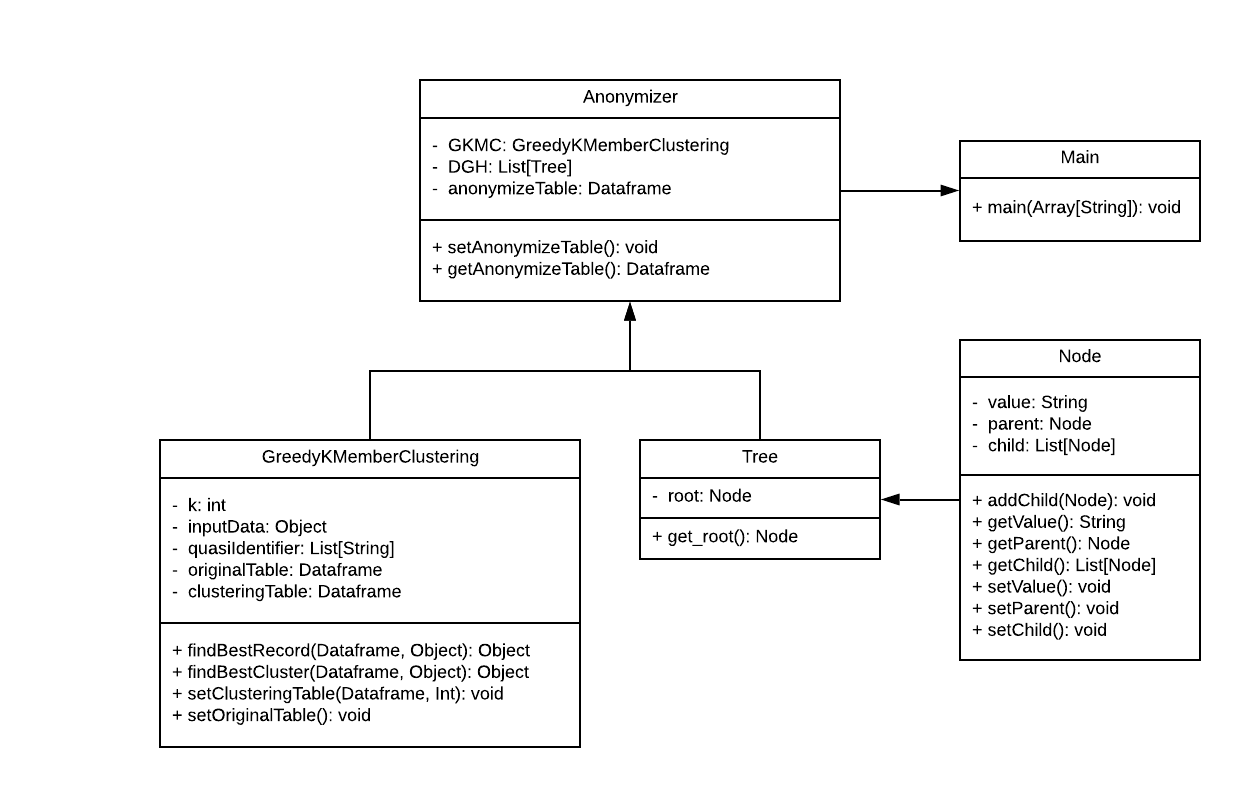
\includegraphics[scale=0.8]{diagram_kelas}
	\caption{Diagram Kelas Anonimisasi Data}
	\label{fig:diagram_kelas}
\end{figure}

Diagram kelas bertujuan untuk menggambarkan keterhubungan antar kelas. Pada penelitian ini digambarkan diagram kelas untuk perangkat lunak anonimisasi data. Karena perangkat lunak analisis data hanya memiliki satu kelas saja, maka keterhubungan antar kelas tidak perlu digambarkan dalam diagram kelas. Gambar \ref{fig:diagram_kelas} menggambarkan keterhubungan antar kelas pada perangkat lunak anonimisasi data. Berikut adalah penjelasan lengkap mengenai deskripsi kelas dan method pada perangkat lunak anonimisasi data:

\begin{itemize}
\item Kelas \textit{Anonymizer} bertujuan untuk melakukan proses anonimisasi setelah data dikelompokan menjadi beberapa \textit{cluster}. Kelas \textit{Anonymizer} memiliki 2 jenis variabel, yaitu:

\begin{itemize}

\item \textit{GKMC} adalah objek dari kelas \textit{GreedyKMemberClustering} yang berisi tabel hasil pengelompokan data berdasarkan algoritma \textit{Greedy k-member clustering}.

\item \textit{DGH} adalah array 1 dimensi dari objek \textit{Tree} yang berisi hasil anonimisasi untuk nilai quasi-identifier yang unik agar menjadi nilai yang lebih umum.

\item \textit{anonymizeTable} adalah array 2 dimensi dari kelas Object untuk menyimpan tabel hasil anonimisasi data.

\end{itemize}

\noindent Kelas \textit{Anonymizer} memiliki 2 jenis method, yaitu:

\begin{itemize}

\item \textit{setAnonymizeTable()} bertujuan untuk melakukan proses anonimisasi pada masing-masing baris data yang tergabung dalam sebuah \textit{cluster}, berdasarkan perbedaan nilai dari beberapa \textit{quasi-identifier}.

\item \textit{getAnonymizeTable()} bertujuan untuk mengambil nilai pada atribut \textit{anonymizeTable}.

\end{itemize}


\item Kelas \textit{GreedyKMemberClustering} bertujuan untuk melakukan pengelompokan data menjadi beberapa \textit{cluster} berdasarkan sifat/nilai atribut yang dimiliki oleh masing-masing baris data. Kelas \textit{GreedyKMemberClustering} memiliki 5 jenis variabel, yaitu:

\begin{itemize}

\item \textit{k} adalah variabel bertipe \textit{Integer} untuk membatasi jumlah anggota pada sebuah \textit{cluster} agar memiliki jumlah yang tetap sebanyak jumlah tertentu.

\item \textit{inputData} adalah variabel untuk menyimpan seluruh baris data \textit{file} CSV.

\item \textit{quasiIdentifier} adalah daftar dari nama-nama kolom yang akan dipilih untuk membuat tabel baru yang digunakan pada proses anonimisasi data

\item \textit{originalTable} adalah tabel yang menyimpan seluruh baris data pada file CSV berdasarkan jenis kolom yang terpilih pada variabel \textit{quasiIdentifier}.

\item \textit{clusteringTable} adalah tabel yang menyimpan hasil pengelompokan baris data dari algoritma \textit{Greedy k-member clustering}.

\end{itemize}

\noindent Kelas \textit{GreedyKMemberClustering} memiliki 4 jenis method, yaitu:

\begin{itemize}
\item \textit{findBestRecord()} bertujuan mencari sebuah baris data yang memiliki nilai \textit{information loss} yang paling minimal dengan baris data lainnya. 

\item \textit{findBestCluster()} bertujuan mencari sebuah \textit{cluster} data yang memiliki nilai \textit{information loss} yang paling minimal dengan \textit{cluster} lainnya.

\item \textit{setClusteringTable()} bertujuan mengelompokkan data berdasarkan algoritma \textit{Greedy k-member clustering} dan hasilnya disimpan pada variabel \textit{clusteringTable}.

\item \textit{setOriginalTable()} bertujuan mengubah hasil pembacaan data input CSV menjadi tabel baru dan hasilnya disimpan pada variabel \textit{originalTable}.

\end{itemize}

\item Kelas \textit{Tree} bertujuan untuk membuat pohon generalisasi berdasarkan jenis atribut \textit{quasi-identifier} yang dipilih.

\item Kelas \textit{Node} bertujuan untuk menyimpan seluruh nilai \textit{quasi-identifier} yang unik untuk masing-masing baris data.

\item Kelas \textit{Main} bertujuan untuk membuat tahapan anonimisasi dari awal sampai akhir dengan memanfaatkan pemanggilan \textit{method} dari masing-masing objek kelas.

\end{itemize}


\begin{figure}[H]
	\centering
	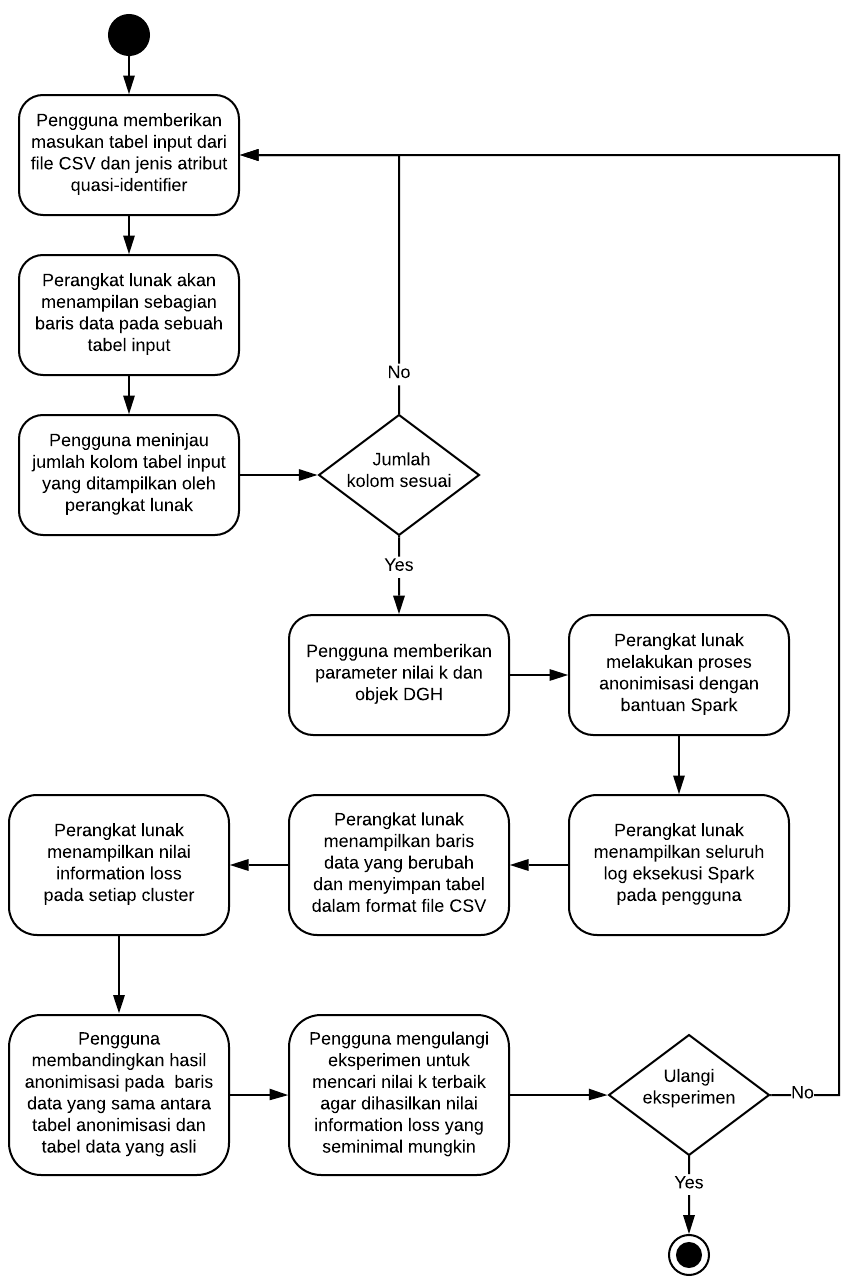
\includegraphics[scale=0.8]{pl_anonimisasi}
	\caption{Diagram Aktifitas Anonimisasi Data}
	\label{fig:pl_anonimisasi}
\end{figure}

\begin{figure}[H]
	\centering
	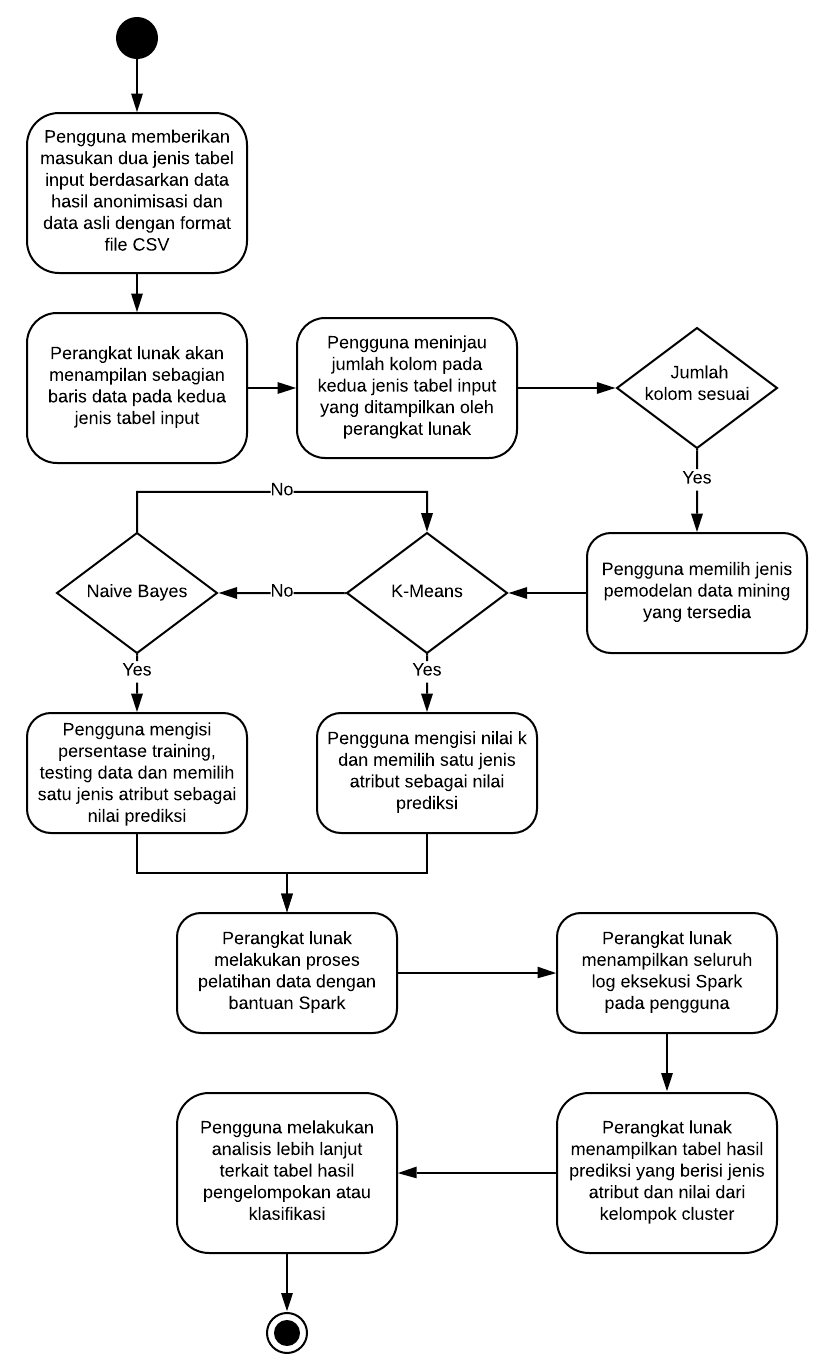
\includegraphics[scale=0.8]{pl_analisis}
	\caption{Diagram Aktifitas Analisis Data}
	\label{fig:pl_analisis}
\end{figure}